%Intro-Teil
% Following the template unter www.hsr.ch > HSR-intern > Bachelor-Studiengänge
% > Informatik > allgemeine Infos Diplom-, Bachelor- und Studienarbeiten.

\newgeometry{left=2.25cm, right=2.25cm, top=2.25cm, bottom=2.25cm} % new
% margins

\begin{titlepage}

\begin{center}
\begin{minipage}[t]{0.45\textwidth}
    
\includegraphics[width=\textwidth]{start/img/hsrLogo}
\end{minipage}
\hspace{\fill} % horizontal space
\begin{minipage}[t]{0.45\textwidth}
    \vspace{-3.26cm}
    
\includegraphics[width=\textwidth]{start/img/ifsLogo} %TODO: more highres logo
\end{minipage}

\end{center}

\vspace{15ex} % vertical space
\begin{center}
	\Huge 
	\begin{framed}
		\textbf{\titel}
	\end{framed}
	
	\vspace{3ex}
	\textbf{\work}
	
	\vspace{1ex}
	\LARGE 
	\place
	
	\vspace{5ex}
	\begin{framed}
		\timeperiod
	\end{framed}
\end{center}

\vspace{11ex}
\begin{tabular}{ll} % Table
	Authoren:        & \authors    \\
	Betreuer:        & \advisor    \\
	Experte:         & \experte    \\
	Gegenleser:      & \gegenleser \\
\end{tabular}

\end{titlepage}

\restoregeometry % reset page margins

% Der Abstract richtet sich an den Spezialisten auf dem entsprechenden Gebiet
% und beschreibt daher in erster Linie die (neuen, eigenen) Ergebnisse und
% Resultate der Arbeit. Es umfasst nie mehr als eine Seite, typisch sogar nur
% etwa 200 Worte (etwa 20 Zeilen). Es sind keine Bilder zu verwenden.

\chapter*{Abstract}\addcontentsline{toc}{chapter}{Abstract}

Die Firma Fluxron Solutions AG mit Sitz in Amriswil stellt Heizlösungen und Küchengeräte auf Induktionsbasis her. Diese Geräte besitzen eine Bluetooth-Schnittstelle, über welche die Einstellungen angepasst werden können. Zudem bietet die Schnittstelle eine ausführliche Laufzeit- und Fehlerprotokollierung an. Servicetechniker benötigen genau diese Informationen zur Fehlersuche und Reparatur der Geräte in Grossküchen. Aufgrund der grossen Anzahl Geräte, ist es schwierig die Installationen im Überblick zu behalten.

In dieser Arbeit wurde eine Applikation für Android entwickelt, welche von den Technikern zur Diagnose und Konfiguration genutzt werden kann. Die Lage der verbauten Geräte wird auf Situationsfotos markiert. Damit kann bei einem Serviceeinsatz die Position und der Status aller Kochinstallationen angezeigt werden.

Zur Umsetzung des Projektes wurden agile Softwareentwicklungsmethoden eingesetzt. Neben einer gründlichen Anforderungsanalyse wurde die Benutzeroberfläche mit Mockups konzipiert und mittels Usability Walkthroughs validiert.

Als Programmiersprache wurde Java 7 für Android eingesetzt. Die Anwendungsarchitektur besteht aus drei Layern, welche mittels Messages über ein Event Bus System kommunizieren. Um eine zeitgemässe Benutzeroberfläche zu erstellen, wurde diese im schlichten aber effektiven Material Design umgesetzt. Lokal werden die Daten in einer dokumentbasierten Datenbank gespeichert. Die Kommunikation mit den Geräten erfolgt über das CANopen Protokoll. Darüber hinaus bietet die Anwendung konzeptionelle Unterstützung für eine Anbindung an ein Cloud-Backend.

Der Funktionsumfang der Mobilapplikation umfasst die Verwaltung mehrerer Küchen und der darin verbauten Geräte. Küchen können zur besseren Übersicht in einzelne Bereiche unterteilt werden. Die Geräte eines Bereichs werden regelmässig zur Statusaktualisierung abgefragt. \todo{V1 - AKTUALISIERUNG NÖTIG!}
% Das Management Summary richtet sich in der Praxis an die "Chefs des Chefs", d.
% h. an die Vorgesetzten des Auftraggebers (diese sind in der Regel keine
% Fachspezialisten).
% Die Sprache soll knapp, klar und stark untergliedert sein.
% Zu verwenden ist folgenden Gliederung:
% - Ausgangslage - Vorgehen, Technologien - Ergebnisse - Ausblick (optional)

\chapter*{Management Summary}\addcontentsline{toc}{chapter}{Management Summary}

    Todo Einleitung

\textbf{Motivation}

    Todo Motivation
    
\textbf{Ziele}

    Todo Ziele
    
\textbf{Resultate}

    Todo Resultate

\chapter*{Erklärung der Eigenständigkeit}

Hiermit erklären wir,

\begin{itemize}
\item dass wir die vorliegende Arbeit selber und ohne fremde Hilfe durchgeführt haben, ausser derjenigen, welche explizit in der Aufgabenstellung erwähnt sind oder was mit dem Betreuer schriftlich vereinbart wurde,

\item dass wir sämtliche verwendeten Quellen erwähnt und gemäss gängigen wissenschaftlichen Zitierregeln korrekt angegeben haben und,

\item dass wir keine durch Copyright geschützten Materialien (z.B. Bilder) in dieser Arbeit in unerlaubter Weise genutzt haben.
\end{itemize}


Rapperswil-Jona, \today
\\
\\

\includegraphics[width=3cm]{start/img/unterschrift_kkayed} \\*
Konstantin Kayed
\\
\\

\includegraphics[width=3cm]{start/img/unterschrift_twinter} \\*
Theodor Winter

%TODO: Selbststaendigkeitserklaerung als pdf unter start/erklaerung includen.
%\includepdf[pages=-, pagecommand={},
%scale=0.73, trim=80 210 80 80]{start/erklaerung}

%TODO: Index auf Deutsch
\addcontentsline{toc}{chapter}{Inhaltsverzeichnis}
\tableofcontents

%Hauptteil here
% Index of /analysis/

\chapter{Analyse}
\label{chap:Analyse}

% Ausgangslage (Ist-Analyse)

\section{Ausgangslage}
\label{sec:Ausgangslage}

\subsection{Anwendungsumfeld}
\label{subsec:Anwendungsumfeld}

%TODO
% Freistellen
\piccaption{Induktionsherd}
\parpic{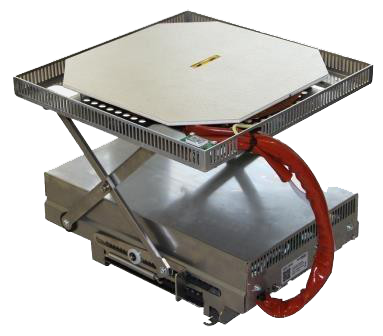
\includegraphics[scale=0.4]{analysis/res/einbaugeraete}}
Die Firma Fluxron AG mit Sitz in Amriswil TG bietet induktive Heiz- und Energiesysteme für Grossküchen an. Die Produktpalette besteht aus verschiedenen Induktionsherden und Thermostatsystemen. Diese haben jeweils ein Bluetoothmodul eingebaut, welches auf ein CANopen-basiertes Protokoll zur Kommunikation setzt. Die Module liefern neben den Geräteeinstellungen auch Fehlercodes und Sensormesswerte via Blootooth.
\picskip{0}
Fluxron verkauft diese Induktionsgeräte an Servicefirmen, welche diese dann beim Endkunden, z.B. einem Restaurant, einbauen und installieren. Dabei, aber auch bei Wartungsarbeiten, setzen die Servicefirmen die bestehende Android Applikation \enquote{FLX Tool} zur Diagnose und zur Konfiguration ein.

Neben den Servicefirmen, setzen auch die Mitarbeiter der Firma Fluxron die Androidapplikation bei internen Versuchen oder zur Ferndiagnose ein. Bei der Ferndiagnose wird eine Teamviewer-Verbindung auf das Smartphone oder den PC des Technikers aufgebaut. Über diese kann dann eine Diagnose mittels den Tools via Bluetooth erfolgen.

\subsection{Bestehende Android-Applikation - Fluxron Systemkonfigurator }
\label{subsec:Bestehende Smartphone-Applikation}
In Eigenentwicklung wurde bei Fluxron bereits eine einfache Android-Applikation entwickelt. Diese unterstützt bereits das Suchen von Geräten, sowie das Lesen und Schreiben von Parametern. Da diese App allerdings immer nur ein Gerät gleichzeitig bedienen kann und die Benutzerinteraktion daher sehr Zeitaufwändig ist, soll im Rahmen dieses Projektes eine neue, übersichtlichere Androidapplikation entstehen. In den nachfolgenden Abschnitten sind die Funktionen dieser Applikation aus funktioneller Sicht aufgelistet.

%TODO Screenshots

\subsubsection{Installation und Konfiguration}
\label{subsubsec:Installation und Konfiguration}
Die App kann ist öffentlich im Google Play Store erhältlich. Nach dem Download muss der Benutzer aber ein Kennwort eingeben, um Zugang zur App und den Gerätefunktionen zu erhalten.

\subsubsection{Verbindungsaufbau zu einem Gerät}
\label{subsubsec:Verbindungsaufbau zu einem Gerät}
Um eine Verbindung mit einem Gerät herzustellen, muss dieses zuerst über einen Suchlauf gefunden werden. Der Suchlauf zeigt alle momentan aktiven Geräte in einer Liste mit ihrer Device-ID an. In der Liste sind neben den aktiven Geräten auch alle Geräte aufgelistet, welche schon einmal mit der App verbunden waren.

Danach kann man sich mit einem Gerät aus der Liste verbinden um mit dem Gerät zu interagieren.

\subsubsection{Statusansicht}
\label{subsubsec:Statusansicht}
Wenn ein Gerät verbunden ist, kann der Benutzer über die entsprechende Schaltfläche zum Gerätetyp zu der Statusübersicht des Gerätes gelangen. Auf der Statusübersicht kann der Benutzer u.a. folgende Informationen auslesen:
\begin{itemize}
\item Statuscode
\item Temperatur des Kühlkörpers
\item Temperaturgradient
\item Pfannenerkennung
\item Soll- und Ist-Temperaturen der einzelnen Zonen
\item Leistungsaufnahme
\end{itemize}

\subsubsection{Setupansicht}
\label{subsubsec:Setupansicht}
Wenn ein Gerät verbunden ist, kann in der Setupansicht eine Liste aller Parameter des Gerätes ausgelesen werden. Der Benutzer kann Parameter anwählen, eine kurze Beschreibung dazu ansehen und deren Werte ändern.

\subsubsection{Historyansicht}
\label{subsubsec:Ansichten}
In der Historyansicht können Betriebszähler eingesehen. Dies beinhaltet Werte wie z.B. die Anzahl von "Power-On" Events oder Laufzeit des Gerätes.

Neben den Zähler kann ein Fehlerlog eingesehen werden, welches die letzten Zehn Fehlercodes beinhaltet. Dies kann zur Diagnose von Problemen sehr hilfreich sein.

\subsubsection{Einschränkungen der App}
\label{subsubsec:Einschränkungen der App}
\begin{itemize}
\item Es kann immer nur ein Gerät gleichzeitig verbunden sein
\item Für jede Verbindung ist ein erneuter Suchlauf nötig
\item Die Geräte sind nur mit der ID sichtbar, dies macht die Orientierung in einer Grossküche mit einem dutzend Geräten schwierig
\item Wenn ein nicht verbundenes Gerät eine Fehlermeldung absetzt, wird diese nicht empfangen
\item Typ der verbundenen Geräte wird zwar erkannt, die Benutzeroberfläche bietet aber immer noch alle Gerätetypen an
\end{itemize}

\subsection{Weitere bestehende Software}
\label{subsec:Weitere bestehende Software}
\subsubsection{FLX Access}
\label{subsubsec:FLX Access}
\piccaption{FLX Access}
\parpic{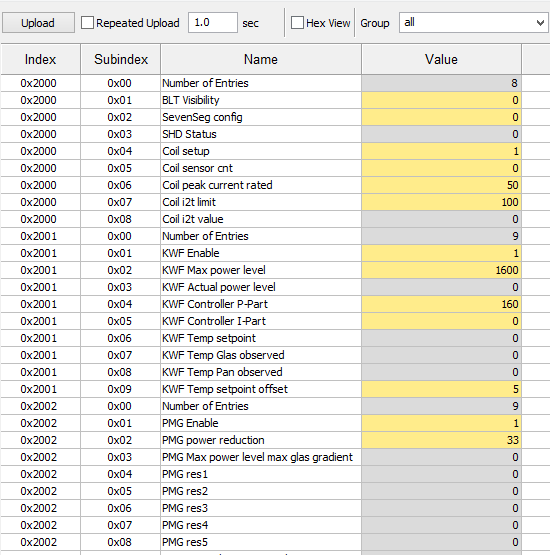
\includegraphics[scale=0.4]{analysis/res/flxaccess}}
Mit FLX Access stellt Fluxron ein Windows-Tool zum auslesen und setzen von gerätespezifischen Parametern bereit. Die Kommunikation erfolgt via Bluetooth. Zudem kann der Gerätestatus ausgelesen werden. 

Dieses System ist besonders für die Entwicklungsphase von Geräten gedacht.
\picskip{0}
\subsubsection{FLX Downloadtool}
\label{subsubsec:FLX Downloadtool}

\piccaption{FLX Access}
\parpic{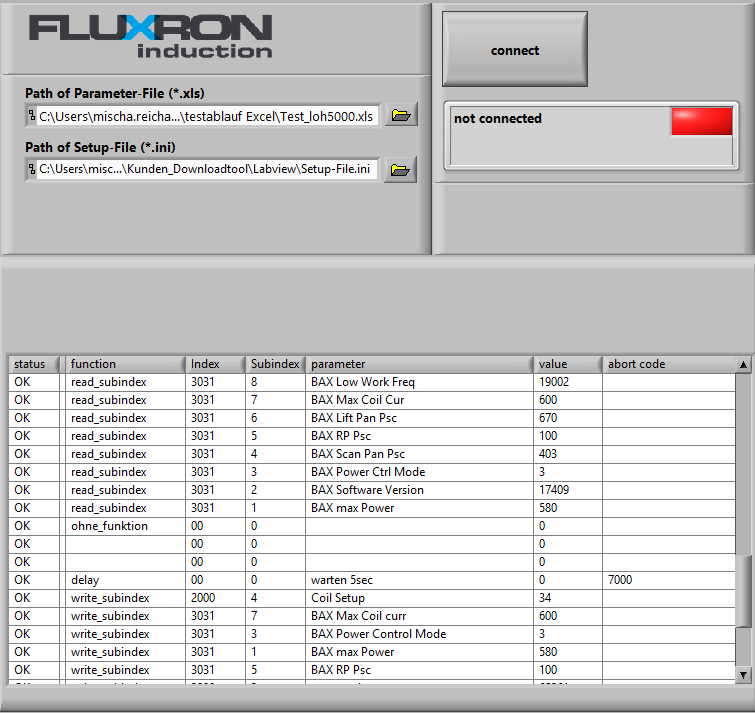
\includegraphics[scale=0.25]{analysis/res/flxdltool}}
Das FLX Downloadtool ermöglicht den Download der gesamten Konfiguration in eine Excel-Datei. In dieser können dan die Parameter eingestellt werden. Danach werden die Einstellungen über das Tool wieder auf das Gerät geladen.

Eingesetzt wird dieses Programm für das Schreiben von kundenspezifischen Parametern auf mehrere Geräte.
\picskip{0}

% NFR

\section{Non Functional Requirements}
\label{sec:Non Functional Requirements}

\begin{itemize}
\item Die Applikation soll 30 - 50 Fluxron Geräte problemlos verwalten können. In einzelnen Spezialfällen kann es aber bis zu 150 Geräte geben. Die App sollte damit ebenfalls umgehen können, allerdigs sind leichte Einschränkungen kein Problem.
\item Die Applikation soll modular aufgebaut sein, so dass zukünftige Erweiterungen leicht realisiert werden können.
\item Der Code soll so dokumentiert werden dass eine Weiterentwicklung der Applikation durch die FLUXRON Solutions AG möglich ist.
\item Die Applikation soll auf Android Geräten die bis zu 2 Jahre alt sind lauffähig sein.
\item Sowohl Bluetooth Classic als auch Bluetooth 4.0 sollen von der Applikation unterstützt werden.
\item Die Applikation soll so einfach bedienbar sein dass keine Schulung der Benutzer erforderlich ist.
\item Die Applikation soll auch ohne bestehende Internet-Verbindung vollständig funktionsfähig sein.
\end{itemize}


\subsection{Anforderungen an Android-Version}
\label{subsec:Non Functional Requirements}
Aufgrund der alten Produktgeneration muss die App auf einer Android-Version laufen, welche klassische Bluetoothverbindungen unterstützt. Zudem sollte die App auch auf einer neuen Version von Android mit Bluetooth 4.0 \ac{LE} betrieben werden können.

Bluetooth 4.0 unterstützt sowohl klassische Bluetoothverbindungen, als auch die neuen Low Energy Verbindungen. Die klassichen Verbindungen sind rückwärtskompatibel mit den Vorgängerwersionen.\cite{bt_standard}

Android unterstützt Bluetooth 4.0 (inklusive \ac{LE}) ab der API-Version 4.3\cite{bt_android}. Dies ist somit die minimal nötige Version, um die Kompatibilität zu gewährleisten.

Mit der Auswahl der Version 4.3 (Android JellyBean) können somit mehr als 50\% der momentan im Umlauf \cite{android_distribution} befindlichen Geräte unterstützt werden.
% Index of /projectmanagement/

\chapter{Projektmanagement}
\label{chap:Projektmanagement}

% Risikomanagement

\section{Risikomanagement}
\label{sec:Risikomanagement}

\begin{table}[H]
\begin{tabularx}{\textwidth}{l|>{\raggedright\arraybackslash}X}
\multicolumn{2}{l}{\textbf{R1: Erwartungen des Kunden nicht erfüllt }} \\
\hline
Beschreibung & Die Applikation erfüllt die funktionalen oder gestalterischen Erwartungen des Kunden nicht.\\
\hline
Massnahme & Es wird mit dem Kunden eine wöchentliche Besprechungen per Skype durchgeführt. Dabei wird der aktuelle Stand der Arbeit gezeigt.\\
\hline
Vorgehen beim Eintreffen & Applikation gemäss den Wünschen des Kunden anpassen.
\\
\end{tabularx}
\caption{Risiko - Erwartungen des Kunden nicht erfüllt}
\end{table}

\begin{table}[H]
\begin{tabularx}{\textwidth}{l|>{\raggedright\arraybackslash}X}
\multicolumn{2}{l}{\textbf{R2: Performance reicht nicht für das Verwalten von 100 Geräten }} \\
\hline
Beschreibung & Die Performance der Applikation reicht nicht aus um 100 Fluxron Geräte pro Küche zu verwalten beziehungsweise grafisch darzustellen.\\
\hline
Massnahme & Bei der Entwicklung werden Performance Tests mit bis zu 100 simulierten Fluxron Geräten durchgeführt.\\
\hline
Vorgehen beim Eintreffen & Die maximale Zahl von Geräten pro Küche reduzieren.
\\
\end{tabularx}
\caption{Risiko - Performance reicht nicht}
\end{table}

\begin{table}[H]
\begin{tabularx}{\textwidth}{l|>{\raggedright\arraybackslash}X}
\multicolumn{2}{l}{\textbf{R3: Bluetooth Classic und 4.0 nicht in der gleichen Applikation }} \\
\hline
Beschreibung & Es ist nicht möglich Unterstützung für Bluetooth Classic und 4.0 in der gleichen Applikation anzubieten.\\
\hline
Massnahme & In der Inception Phase wird die Bluetooth Unterstützung von Android recherchiert. Es wird nach Möglichkeit eine Android Version gewählt die beide Bluetooth Standards unterstützt.\\
\hline
Vorgehen beim Eintreffen & Es wird nur Unterstützung für Bluetooth Classic angeboten.
\\
\end{tabularx}
\caption{Risiko - Bluetooth Classic \& 4.0 Unterstützung}
\end{table}

% Meilensteine

\section{Meilensteine}
\label{sec:Meilensteine}


\begin{table}[H]
\begin{tabularx}{\textwidth}{ c | l | X | l}
\textbf{MS} & \textbf{Name} & \textbf{Resultate}  & \textbf{Datum} \\ \hline
MS1 & Kickoff              & Aufgabenstellung & 09.09.2015 \\ \hline
MS2 & Ende Inception       & Infrastruktur, Ausgangslage, Anforderungsspezifikation, Projektplan, Risikomanagement, Use Cases, Testspezifikation, Domainanalyse, Arbeitspakete	& 29.09.2015 \\ \hline
MS3 & Architekturprototyp  & Prototyp	& 13.10.2015 \\ \hline
MS4 & Zwischenpräsentation & Kunde und Experte informiert & 26-31.10.2015 \\ \hline
MS5 & Feature 75\%         & 75\% aller Features erarbeitet & 10.11.2015 \\ \hline
MS6 & Produkt fertig       & Alle geforderten Funktionen der Applikation sind implementiert. & 22.11.2015 \\ \hline
MS7 & Ende Testphase       & Testprotokolle sind vorhanden & 06.12.2015 \\ \hline
MS7 & Abgabe Abstract      & Das Abstract wurde an den Betreuer abgegeben. & 10.12.2015 \\ \hline
MS8 & Abgabe Bericht       & Der Bericht wurde an den Betreuer abgegeben. & 18.12.2015 \\
\end{tabularx}
\caption{Meilensteine}
\end{table}

% Projektplan

\clearpage
\begin{sidewaysfigure}
\section{Projektplan}
\label{sec:Projektplan}
\centering
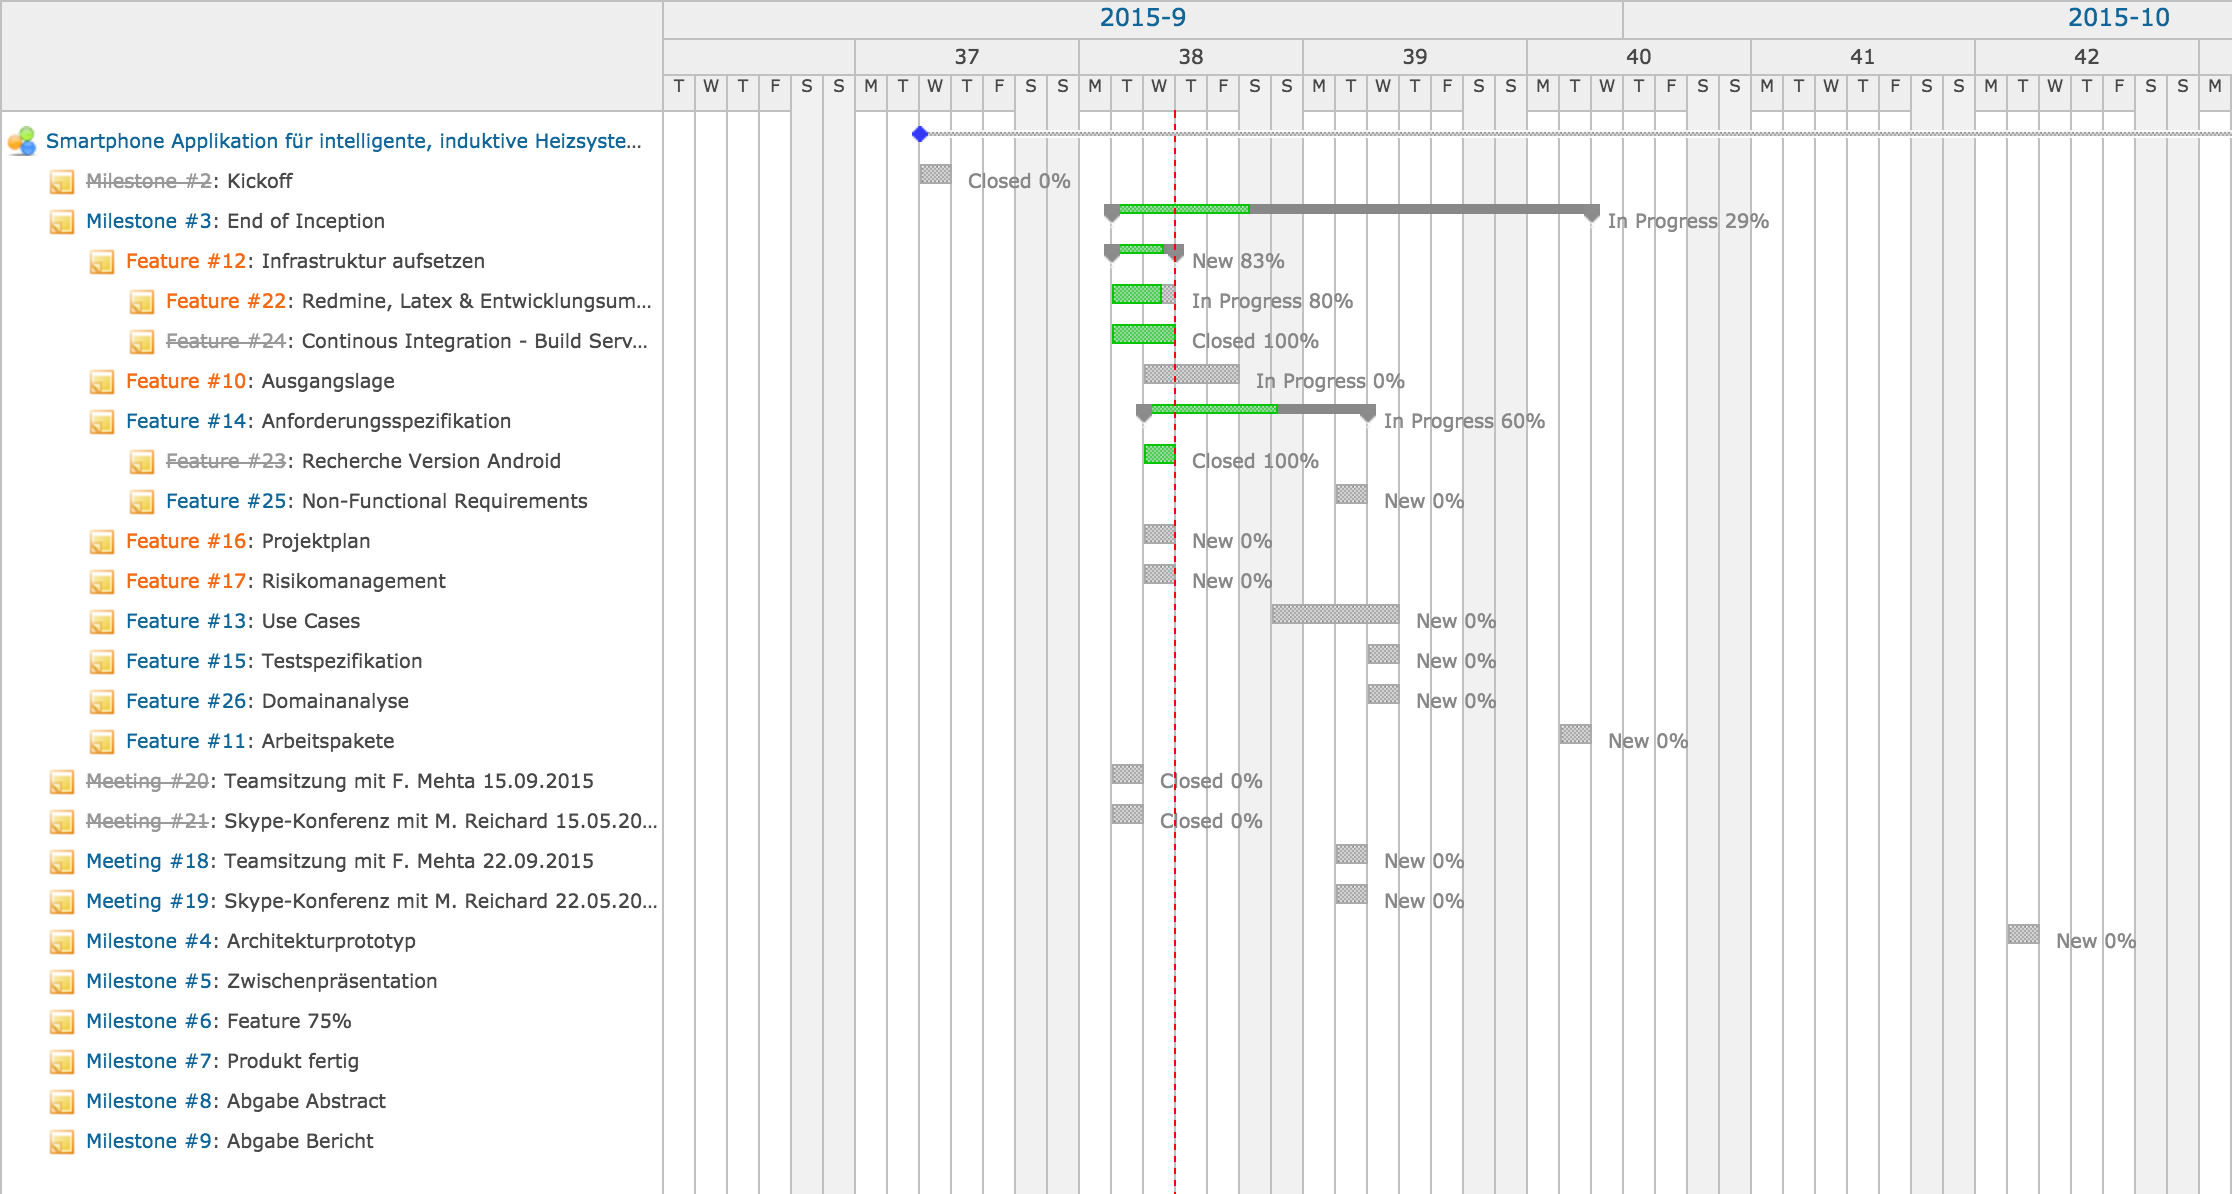
\includegraphics[scale=0.45]{projectmanagement/res/projektplan.png}
\end{sidewaysfigure}
\clearpage
% Index of /design/

\chapter{Konzeption und Design}
\label{chap:Konzeption und Design}

\section{Code Style Guidelines}
\label{sec:Code Style Guidelines}

Um die Zusammenarbeit mit mehreren Personen zu regeln, verwenden wir den folgende Code Style Guide: \url{https://source.android.com/source/code-style.html#java-language-rules}.

Zur Vereinfachung einer späteren Veröffentlichung achten wir von Anfang an auf die Android Launch Checkliste:\\ \url{http://developer.android.com/distribute/tools/launch-checklist.html}.

\subsection{Einschränkungen}
Die folgenden Empfehlungen aus dem Code Style Guide werden wir nicht übernehmen:

\begin{itemize}
\item \textbf{Jedes File hat zuoberst ein Copyright Statement.} \\ Der gesamte Code erhält eine Lizenz welche zentral abgelegt wird. Bei jedem File ein solches Statement einzufügen ist unnötig und wäre redundant.
\item \textbf{Statische Variablen beginnen mit s. Nicht-öffentliche, nicht-statische Variablen beginne mit m. Alle andern werden klein geschrieben.} \\ Diese Konvention ist unnötig da man diese Informationen problemlos auch dem Code entnehmen kann. Moderne IDEs wie Android Studio unterstützen einem dabei zusätzlich durch farbliches Hervorheben. In diesem Projekt werden alle Variablen, ausser Konstanten, klein geschrieben. Konstanten werden vollständig aus Grossbuchstaben zusammengesetzt.
\end{itemize}

\section{UX Guidelines}
\label{sec:UX Guidelines}

Bei der Entwicklung des User Interfaces nutzen wir den Material Design Style Guide:
\url{https://developer.android.com/design/index.html}. Dieser Guide ist eigentlich für Android 5.0 ausgelegt, unsere Applikation muss jedoch von Android 4.3 an lauffähig sein. Daher müssen einige Einschränkungen, z.B. bei der Verwendung von Animationen, in Kauf genommen werden.


\section{Architektur}
\label{sec:Architektur}

\subsection{Rahmenbedingungen}
\begin{figure}[H]
    \begin{center}
    		% GFX Trim left bottom right top
        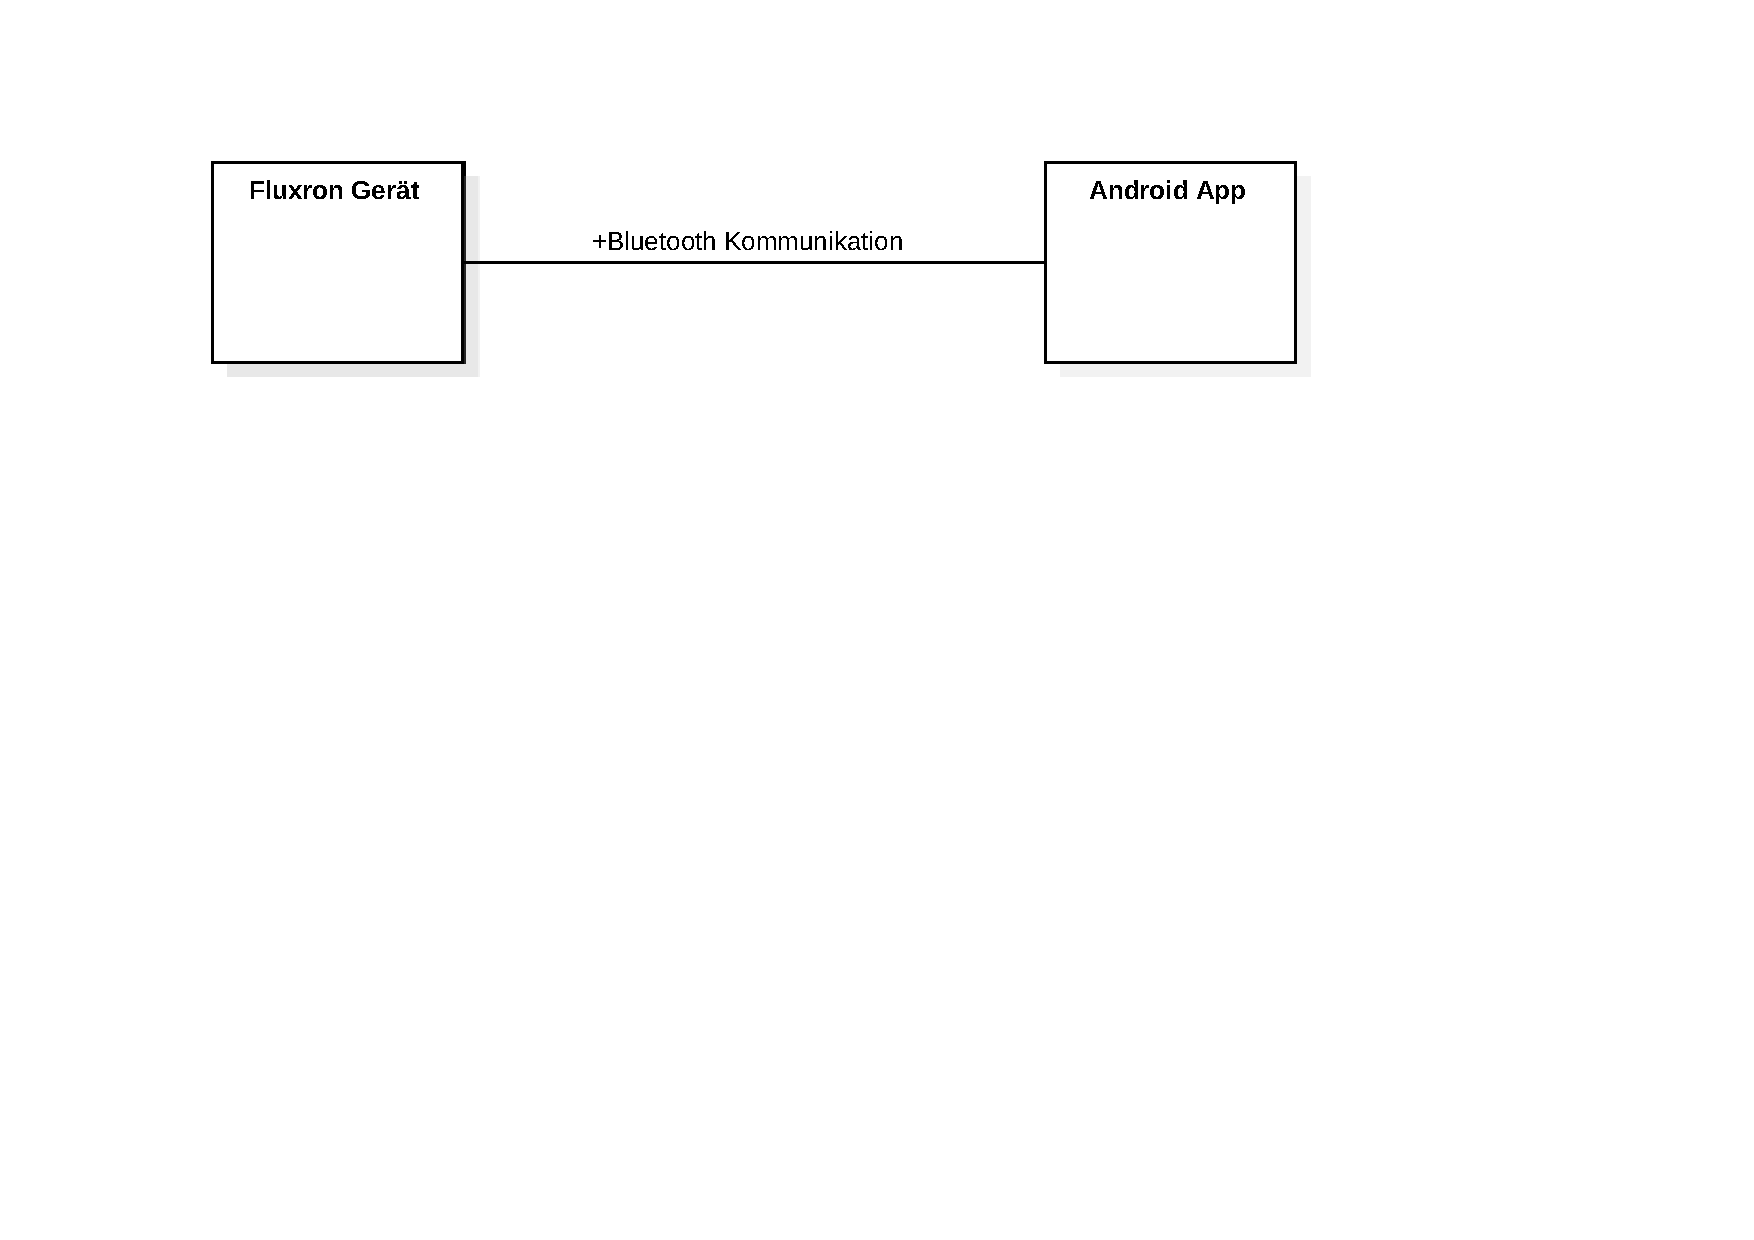
\includegraphics[trim=30 420 140 60,clip,width=\textwidth]{design/res/blackbox}
    \end{center}
    \caption{Blackbox Darstellung}
\end{figure}

Die Applikation kommuniziert mit bis zu 150 Fluxron Geräten via Bluetooth. Auf Grund der Natur von Bluetooth Geräten ist mit einer stark asynchronen Kommunikation zu rechnen. Die Architektur der Fluxron Geräte ist bereits vorgegeben. Die Kommunikation  zwischen den Geräten und der Applikation basiert auf CANopen.

Es soll eine Weiterentwicklung der Applikation durch die \fluxron{} möglich sein.

Die konzeptionellen Anforderungen der \ac{FR}15-18 sowie \ac{NFR}2, 3 sollen durch die Architektur unterstützt werden.

\subsection{Variante A: Schichtenarchitektur}
\begin{figure}[H]
    \begin{center}
    		% GFX Trim left bottom right top
        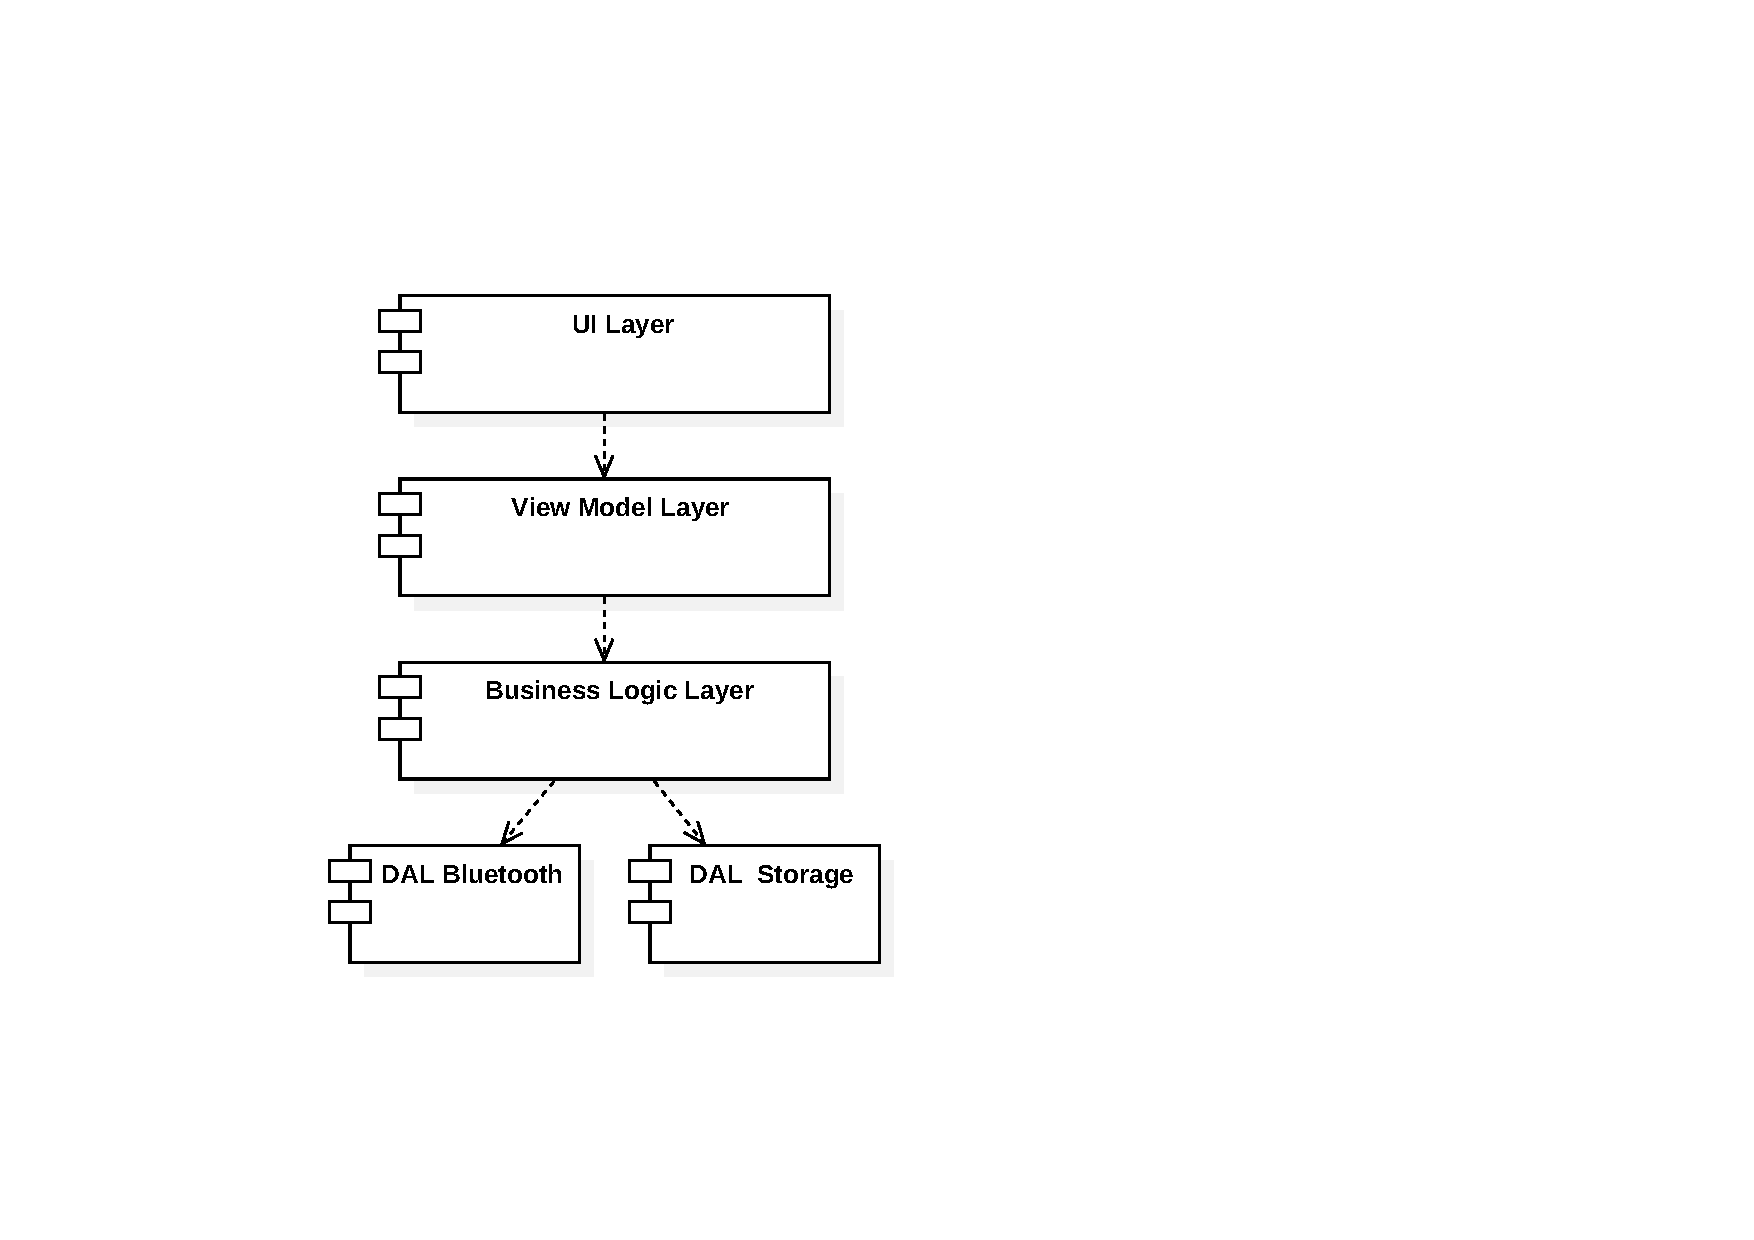
\includegraphics[trim=-100 130 140 110,clip,width=\textwidth]{design/res/layers}
    \end{center}
    \caption{Layer Architektur}
\end{figure}

Die Architektur wird in mehrere Schichten unterteilt. Dabei wird die Kopplung in die Gegenrichtung durch Interfaces und Observer aufgelöst.

\subsection{Variante B: MVC Architektur}
\begin{figure}[H]
    \begin{center}
    		% GFX Trim left bottom right top
        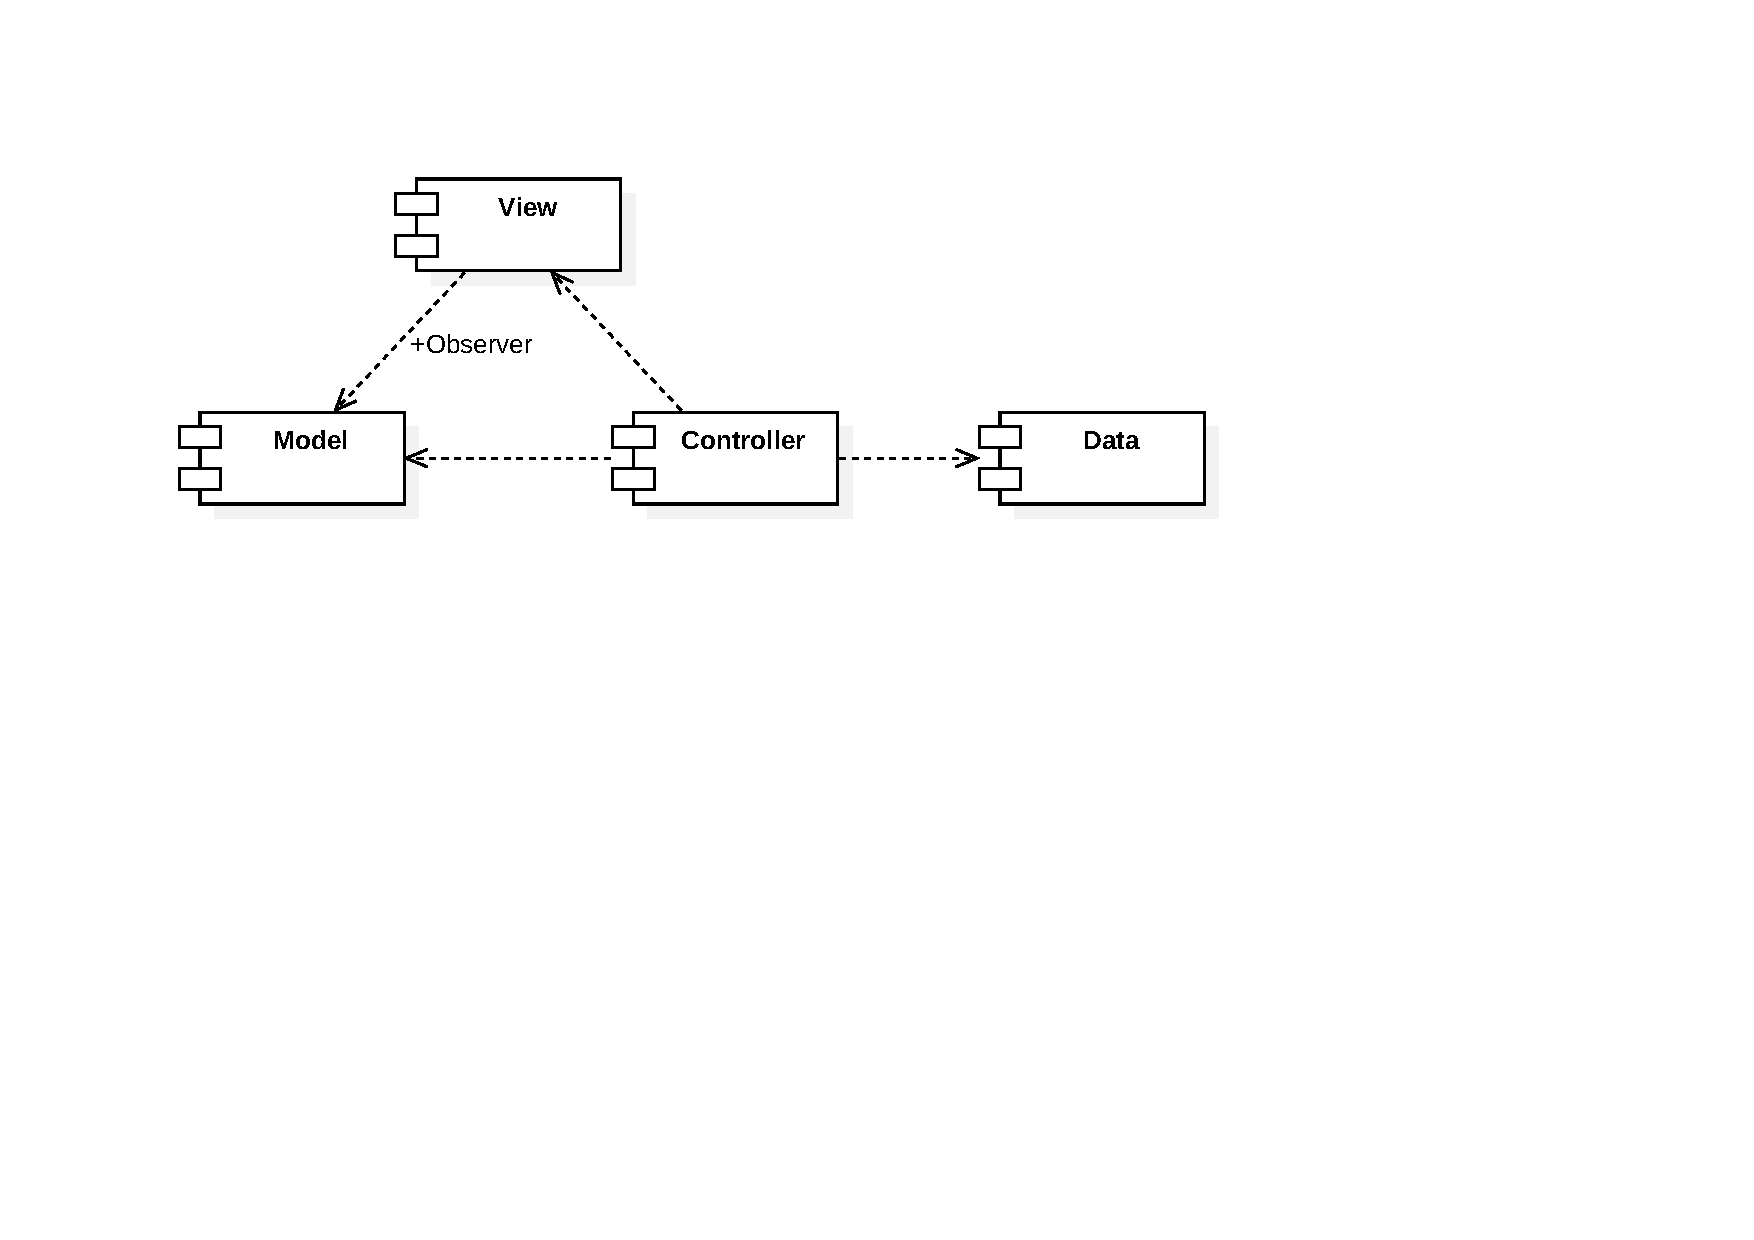
\includegraphics[trim=0 330 140 60,clip,width=\textwidth]{design/res/mvc}
    \end{center}
    \caption{MVC Architektur}
\end{figure}

Weil die Applikation stark durch das User Interface definiert ist, liegt eine Umsetzung mit dem MVC Pattern nahe.

\subsection{Variante C: Event Bus Architektur}
\begin{figure}[H]
    \begin{center}
    		% GFX Trim left bottom right top
        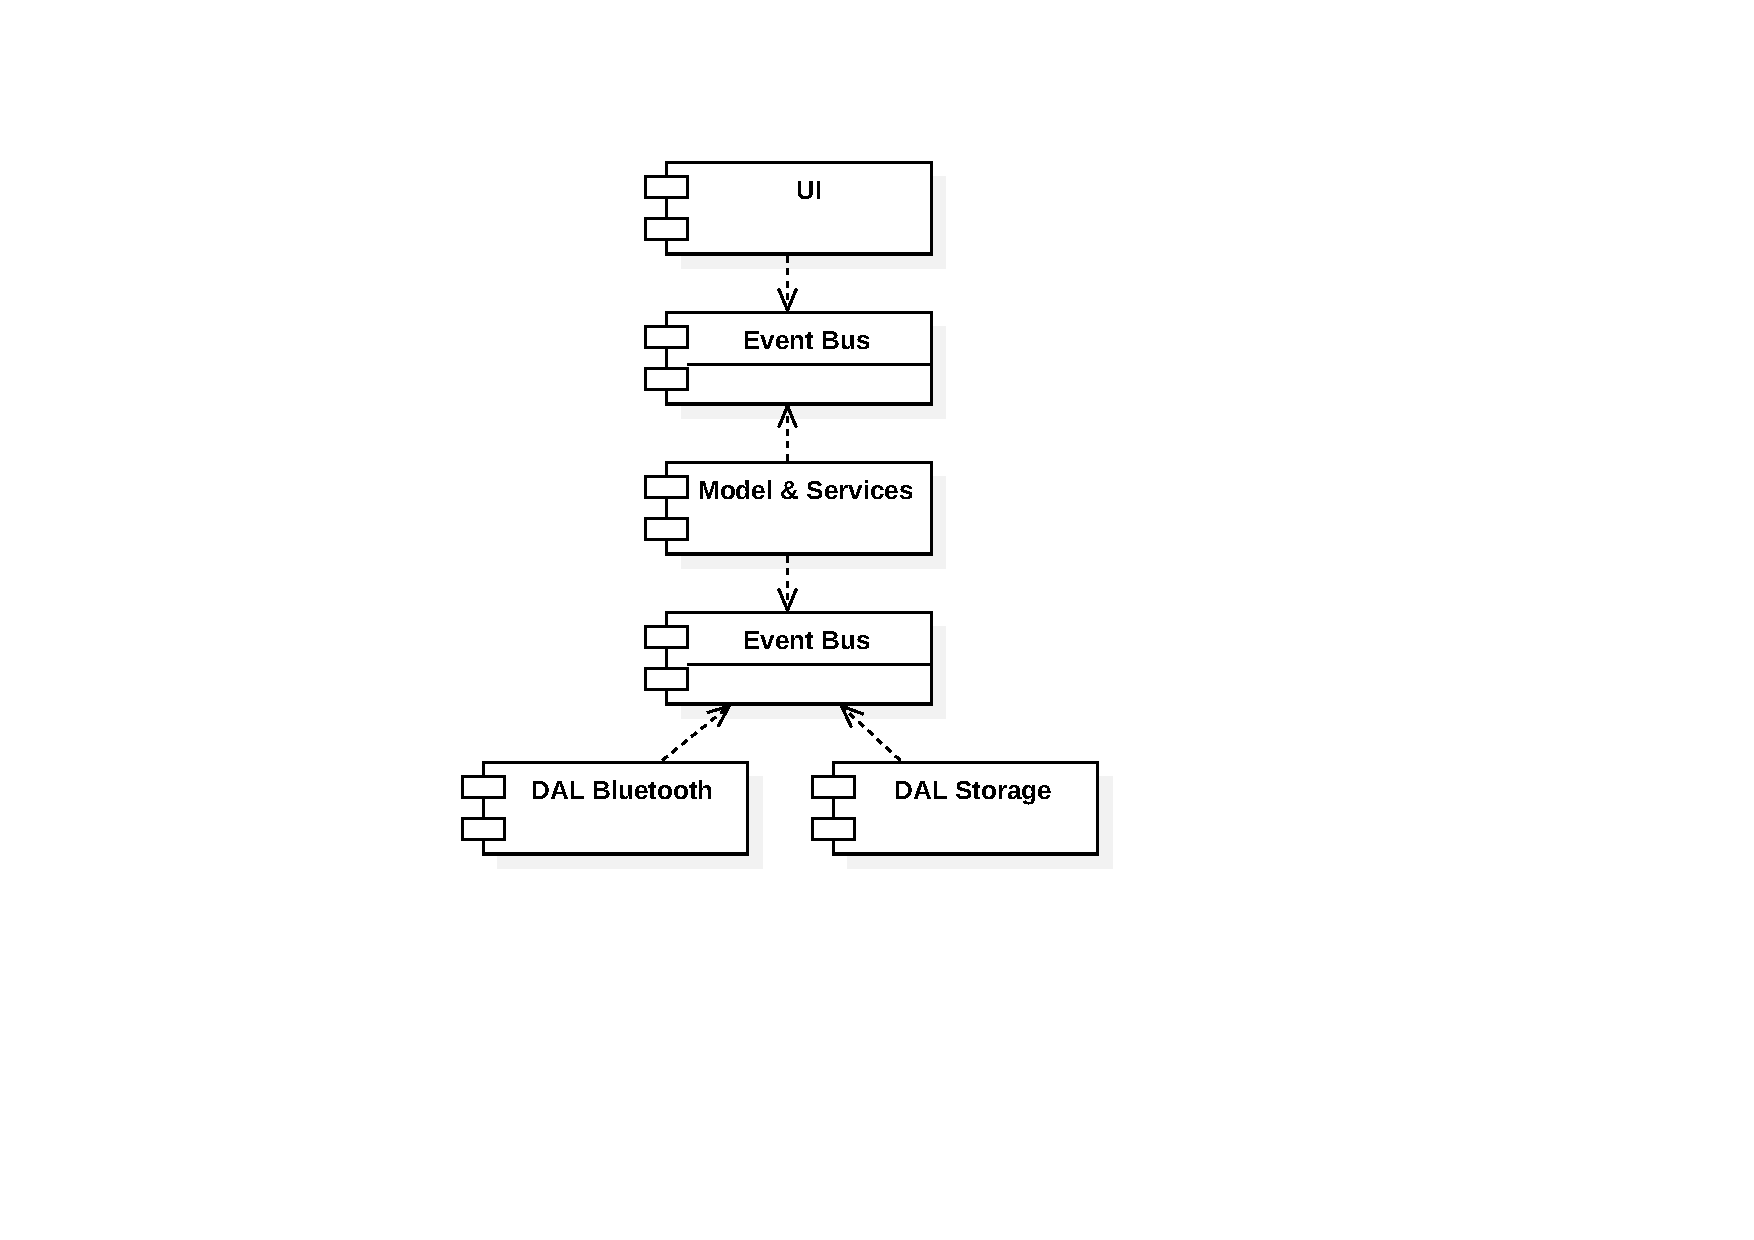
\includegraphics[trim=0 180 100 30,clip,width=\textwidth]{design/res/eventbus}
    \end{center}
    \caption{Event Bus Architektur}
\end{figure}

Mit einem Event Bus zwischen \ac{UI} und Model ist eine stärkere Entkopplung möglich\cite{fowler_event_collab}. Der Event Bus zwischen Model und \ac{DAL} ermöglicht mehrere Module wie Bluetooth und Storage.

\subsection{Bewertung der Architekturmöglichkeiten}

\begin{table}[H]
\begin{tabular}{|p{\textwidth{}/2}|p{\textwidth{}/2}|}
 \hline 
\multicolumn{2}{|c|}{\textbf{Variante A: Schichtenarchitektur}}\\ \hline 
Vorteile
\begin{enumerate}
\item Einfach verständlich, klassische Architektur
\item Separation of Concerns, Low Coupling, High Cohesion
\end{enumerate} & 
Nachteile
\begin{enumerate}
\item \ac{UI} Layer muss ganze Objekthierarchien beobachten
\item Kein einheitliches Parallelitätskonzept
\end{enumerate}
\\ \hline

\multicolumn{2}{|c|}{\textbf{Variante B: MVC Architektur}}\\ \hline 
Vorteile
\begin{enumerate}
\item Gute Entkopplung der View von der Logik
\item Reduktion von Navigationslogik
\end{enumerate} &
Nachteile
\begin{enumerate}
\item \ac{MVC} nur verwendbar in Kombination mit weiteren Patterns
\item Komplexe Observerstruktur zwischen View und Model
\item Kein einheitliches Parallelitätskonzept
\end{enumerate}
\\ \hline

\multicolumn{2}{|c|}{\textbf{Variante C: Event Bus Architektur}}\\ \hline 
Vorteile
\begin{enumerate}
\item Parallelität kann zentral von Bus synchronisiert werden
\item Einfachere Komponenten
\item Flache Observerstruktur im User Interface
\item Einfaches Hinzufügen von zusätzlichen Komponenten
\end{enumerate} &
Nachteile
\begin{enumerate}
\item Auf Grund flacher Hierarchie ist es leicht möglich Separation of Concerns zu verletzen.
\item Komplexere Interaktionslogik (Beispiel Message Chains)
\end{enumerate}
\\ \hline
\end{tabular}
\caption{Bewertung Architekturmöglichkeiten}
\end{table}

\subsubsection{Fazit}
Wir entscheiden uns für Variante C, denn sie ermöglicht uns die gewünschte konzeptionelle Erweiterbarkeit in Hinblick auf die \ac{FR} und \ac{NFR} die in Zukunft noch umgesetzt werden sollen. Zudem ermöglicht diese Architektur die Komplexität der Observer stark zu vereinfachen. Die stark asynchrone Kommunikation wird ideal unterstützt.

\section{Nebenläufigkeitskonzept}
\label{sec:Nebenläufigkeitskonzept}
Das Nebenläufigkeitskonzept bezieht sich auf Architektur Variante C \enquote{Event Bus}.

\subsection{Sicherstellen der Asynchronität}
Um sicherzustellen das alle Ereignisse asynchron verarbeitet werden, muss der Event Bus so konfiguriert werden dass er die Meldungsverarbeitung in einem eigenen Thread durchführt. Dies gilt auch für Meldungen die im \ac{UI}-Thread erzeugt werden. Damit ist sichergestellt das der \ac{UI}-Thread nicht blockiert.

\subsection{Synchronisierung mit \ac{UI}-Thread}
Zugriffe auf das User Interface dürfen nur vom UI-Thread durchgeführt werden. Dazu müssen die Subscriber dem Event Bus den gewünschten Ausführungsthread angeben können.

\subsection{Thread-Safety der Event Bus Subscriber}
Alle Subscribers müssen Sicherstellen (mit Ausnahme UI-Komponenten) dass von mehreren Threads aufgerufen werden können. Dazu werden klassische Java Monitors verwendet. Die Subscribers folgen dem "Run-to-completion" Prinzip.

\subsection{Restart von Activities}
Android kann zur Speicheroptimierung laufende Applikationen (im Hintergrund) ganz oder teilweise beenden. Öffnet der Benutzer die Applikation erneut muss sie ihren Zustand wiederherstellen. Dies erfordert eine Überprüfung dass die Instanzen im Application Context noch vorhanden sind. Gegebenenfalls müssen die Event Busse neu gestartet werden.
% Index of /uiux/

\chapter{UI-/UX-Konzept}
\label{chap:UI-/UX-Konzept}

% Index of /design/

\section{Farben und Formen}
\label{sec:Farben und Formen}

\subsection{Farbgebung}
\label{subsec:Farbgebung}
\begin{figure}[H]
    \begin{center}
    		% GFX Trim left bottom right top
        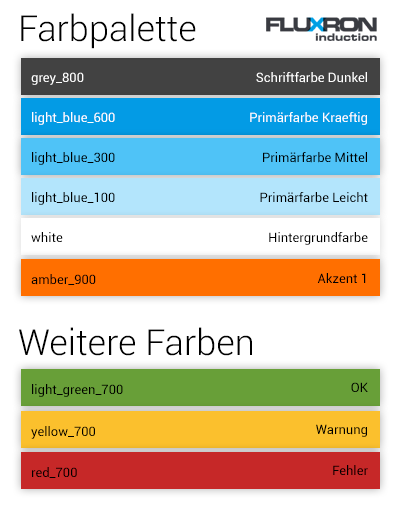
\includegraphics[trim=0 200 0 50,clip,scale=0.7]{uiux/res/basic_colors}
    \end{center}
    \caption{Grundlegende Farben der App}
\end{figure}
Die Farbgebung inspiriert sich am Logo der Firma Fluxron. Ein weisser Hintergrund, mit dunkelgrauer Schrift. Zudem wird ein simples aber aussagekräftiges Komplementärfarbschema zur Hervorhebung spezieller Elemente angewendet.

\subsection{Farben zur Statusanzeige}
\label{subsec:Farben zur Statusanzeige}
\begin{figure}[H]
    \begin{center}
    		% GFX Trim left bottom right top
        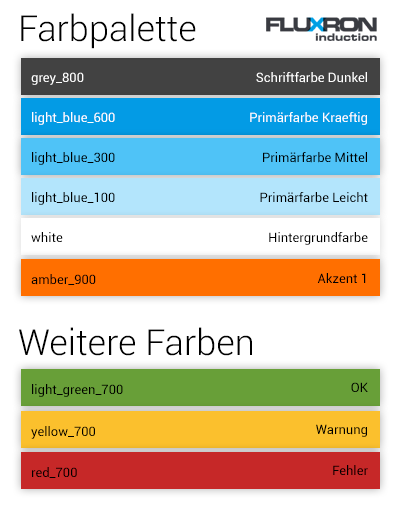
\includegraphics[trim=0 0 0 370,clip,scale=0.7]{uiux/res/basic_colors}
    \end{center}
    \caption{Farben zur Statusanzeige}
\end{figure}
Zur Anzeige von Statusinformationen wird ein klassiches Ampel-Farbschema angewendet. Dieses soll durch die Nutzung von Symbolen unterstützt werden. Diese Farben sollten nur für kleine Flächen genutzt werden.

\section{Navigationskonzept}
\label{sec:Navigationskonzept}

Abbildung \ref{abb:navigationConcept} zeigt das Navigationskonzept für die Mobilapplikation. Zur Navigation verwendet der Benutzer Menüschaltflächen, Listen sowie den Hardwarebutton zur Rückwärtsnavigation (\enquote{Back-Button}).

\begin{figure}[H]
    \begin{center}
    		% GFX Trim left bottom right top
        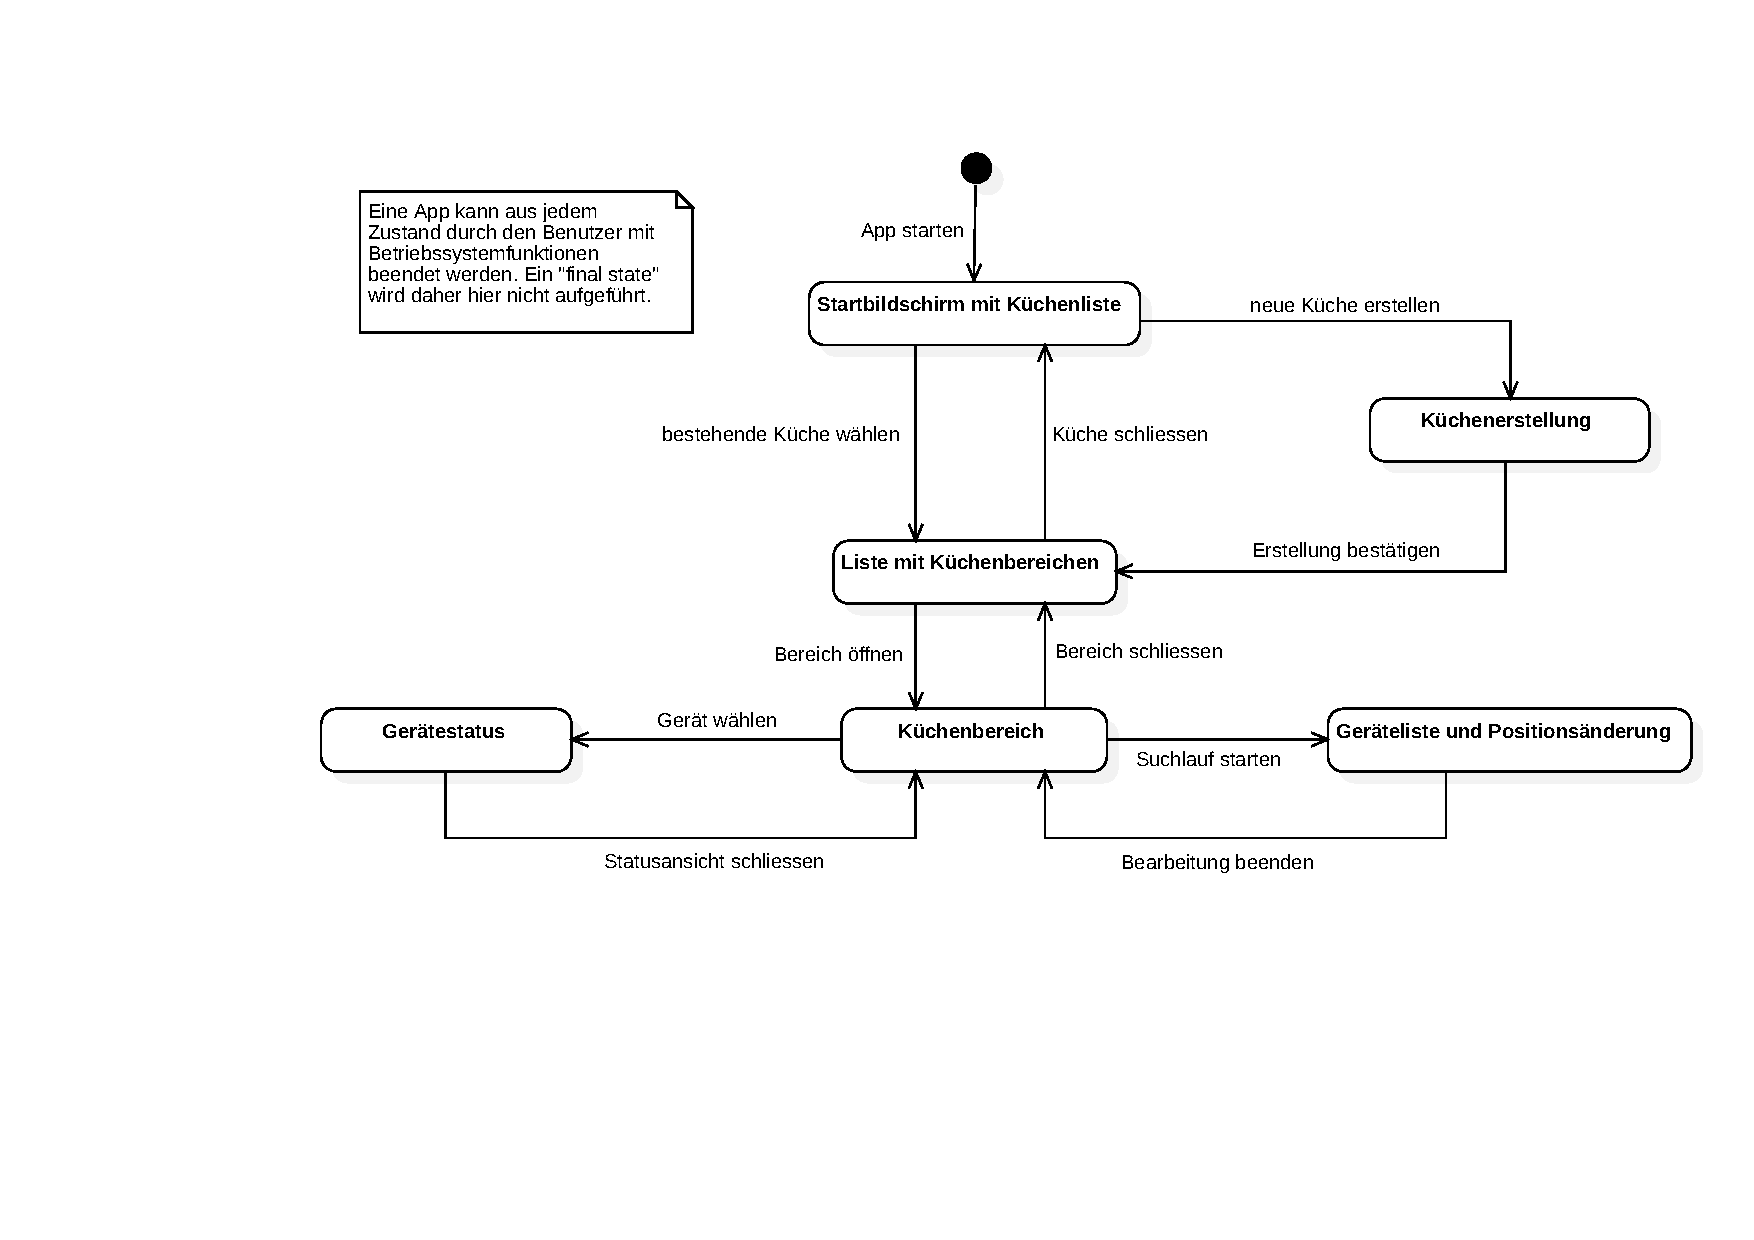
\includegraphics[trim=150 170 0 0,clip,scale=0.6]{uiux/res/navigation}
    \end{center}
    \caption{Farben zur Statusanzeige}
    \label{abb:navigationConcept}
\end{figure}

\vspace{120pt}

% Index of /design/

\section{Mockups}
\label{sec:Mockups}

\subsection{Startbildschirm}
\label{subsec:Startbildschirm}

\begin{wrapfigure}[8]{r}{6cm}
	\begin{center}
		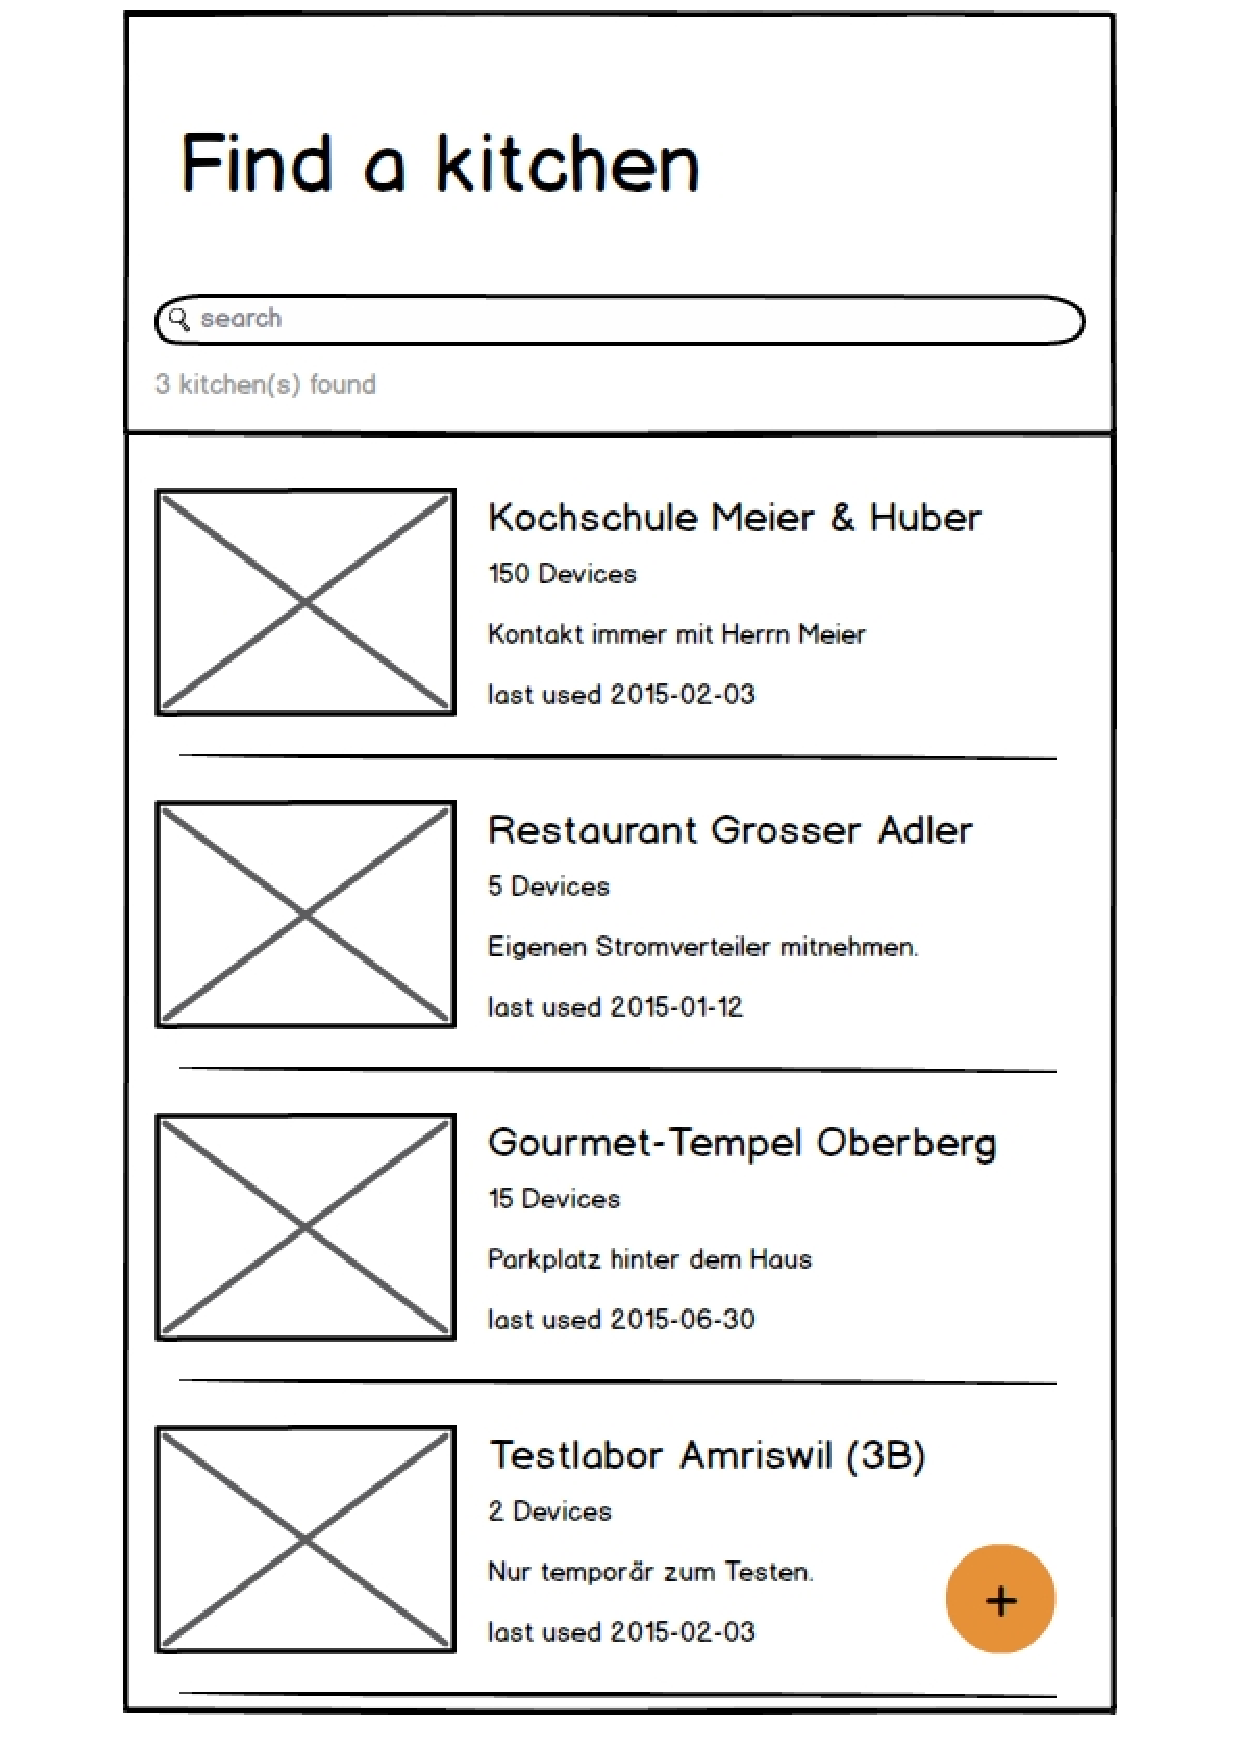
\includegraphics[page=1,trim=0 0 0 0,clip,scale=0.21]{uiux/res/mockups}
		\caption{Mockup Startbildschirm}
	    \label{abb:mockStartScreen}
	\end{center}
\end{wrapfigure}

Der Startbildschirm enthält ein Suchfeld zur einfachen Suche einer Küche nach dem Namen. Darunter werden die Küchen mit ihrem Namen, der Beschreibung und mit der Anzahl Geräte aufgelistet. 

Der Benutzer kann nun eine Küche durch Antippen öffnen, oder mittels dem \ac{FAB} eine neue Küche hinzufügen.

\WFclear
\vspace{3cm}

\subsection{Küchenerstellung}
\label{subsec:Küchenerstellung}

\begin{wrapfigure}[14]{r}{6cm}
	\begin{center}
		\includegraphics[page=2,trim=0 0 0 0,clip,scale=0.21]{uiux/res/mockups}
		\caption{Mockup Küchenerstellung}
	    \label{abb:mockCreateKitchen}
	\end{center}
\end{wrapfigure}

Bei der Küchenerstellung gibt der Benutzer einen Namen für die Küche an. Zudem kann der Benutzer, wenn er möchte, noch eine Beschreibung für diese Küche eingeben.

Zusätzlich sollte der Benutzer auch noch ein Foto von der Küche machen. Damit kann er die Küche später einfacher wiedererkennen. Küchenname und Bild müssen zwingend erfasst werden, die Beschreibung ist nicht erforderlich.

Durch Antippen des \enquote{Create}-Buttons wird die Küche erfasst und der Benutzer auf die Küchenansicht umgeleitet.

\WFclear

\subsection{Küchenbereich mit aktivem Suchlauf}
\label{subsec:Küchenbereich mit aktivem Suchlauf}

\begin{wrapfigure}[12]{r}{6cm}
	\includegraphics[page=4,trim=0 0 0 0,clip,scale=0.21]{uiux/res/mockups}
	\caption{Mockup Küchenansicht}
    \label{abb:mockKitchenView}
\end{wrapfigure}

In der Küchenansicht sieht der Benutzer das Foto für den aktuell gewählten Küchenbereich. Darauf kann er die Geräte aus der Geräteliste platzieren. Die Geräte werden durch einen Kreis, welcher den Status des Gerätes anzeigt, symbolisiert.

Durch Antippen eines Gerätes kann dieses nach Rückfrage gelöscht werden.

Die Geräteliste enthält alle Geräte, welche beim Suchlauf gefunden wurden, oder bereits in der Küche erfasst wurden.

\WFclear

\subsection{Gerätestatus}
\label{subsec:Gerätestatus}

\begin{wrapfigure}{r}{6cm}
	\begin{center}
		\includegraphics[page=5,trim=0 0 0 0,clip,scale=0.21]{uiux/res/mockups}
		\caption{Mockup Gerätestatus}
		\label{abb:mockDeviceDetail}
	\end{center}
\end{wrapfigure}

Die Statusansicht für ein Gerät besteht aus Tabs, zwischen denen der Benutzer mittels Swiping wechseln kann. Für jeden Gerätetyp braucht es hier eine eigene Ansicht da für jede Art von Gerät andere Parameter und Werte relevant sind.

\begin{itemize}
  \item Statusübersicht mit Sensorwerten
  \item Nutzungsstatistik des Geräts
  \item Fehlerhistorie mit letzten 10 Fehlercodes
  \item Einstellungsseite mit Konfigurationsparametern
\end{itemize}

\vspace{6cm}
\WFclear

\subsection{Geräteparameter}
\label{subsec:Geräteparameter}

\begin{wrapfigure}{r}{6cm}
	\begin{center}
		\includegraphics[page=6,trim=0 0 0 0,clip,scale=0.21]{uiux/res/mockups}
		\caption{Mockup Geräteparameter}
		\label{abb:mockDeviceParams}
	\end{center}
\end{wrapfigure}

Die Parameteransicht zeigt eine Liste aller veränderbaren Konfigurationseinstellungen an. Der Benutzer kann die Parameter ändern oder zurücksetzen.

Falls ein Parameter nicht geschrieben werden kann wird eine Fehlermeldung ausgegeben.

Diese Ansicht ist ebenfalls für jeden Gerätetypen unterschiedlich, so haben z.B. Thermostaten mehrere Konfigurationsprofile, die alle in dieser Ansicht bearbeitet werden können.

\WFclear
\vspace{2cm}

\subsection{Nutzungsstatistik}
\label{subsec:Nutzungsstatistik}

\begin{wrapfigure}{r}{6cm}
	\begin{center}
		\includegraphics[page=7,trim=0 0 0 0,clip,scale=0.21]{uiux/res/mockups}
		\caption{Mockup Nutzungsstatistik}
		\label{abb:mockDeviceUsage}
	\end{center}
\end{wrapfigure}

Über die Nutzungsstatistik kann der Benutzer auslesen, wie lange die Werte der Sensoren in den einzelnen Temperaturbereichen lagen. Dies kann zum Beispiel Auskunft über eine fehlerhafte Installation (nicht genügend Wärmeabfuhr am Kühlkörper) Aufschluss geben.

Auch die Statistikseite kann von Gerätetyp zu Gerätetyp variieren.

\WFclear
\vspace{2cm}

\subsection{Fehlerhistorie}
\label{subsec:Fehlerhistorie}

\begin{wrapfigure}{r}{6cm}
	\begin{center}
		\includegraphics[page=8,trim=0 0 0 0,clip,scale=0.21]{uiux/res/mockups}
		\caption{Mockup Fehlerhistorie}
		\label{abb:mockDeviceErrors}
	\end{center}
\end{wrapfigure}

In der Fehlerhistorie werden dem Benutzer die letzten zehn Fehlercodes des Gerätes angezeigt. Diese Bestehen aus einem Fehlercode und einem beschreibenden Text. Zudem wird der Laufzeitzähler des Gerätes zum Fehlerzeitpunkt ausgegeben. Das heisst, für jeden Fehler kann nachgesehen werden, in welcher Laufzeitstunde (ab Installationszeitpunkt) der Fehler aufgetreten ist.

Einzelne Gerätetypen wie z.B. Thermostaten haben weniger oder mehr Fehlercodes in der Historie.

\chapter{Ergebnisse}
\label{chap:Ergebnisse}

\section{Zielerreichung}

\pagebreak
\section{Benutzerhandbuch}

\subsection{Installation}
Um die Applikation zu installieren, muss die .apk Installationsdatei zuerst auf das Smartphone übertragen werden. Danach muss sichergestellt werden, dass in den Android Einstellungen unter Sicherheit die Option \enquote{Unbekannte Herkunft zulassen} aktiviert wurde. Nun kann mit einem gängigen Dateiexplorer die Installationsdatei geöffnet werden um den Installationsvorgang zu beginnen.
\subsection{Logininformationen hinterlegen}

Um die Applikation verwenden zu können, müssen die Login-Informationen des Benutzers hinterlegt werden. Dazu wird direkt nach dem Start der Applikation das Zahnrad im oberen rechten Ecken berührt.

\begin{wrapfigure}{l}{5.5cm}
	\vspace{-0.44cm}
	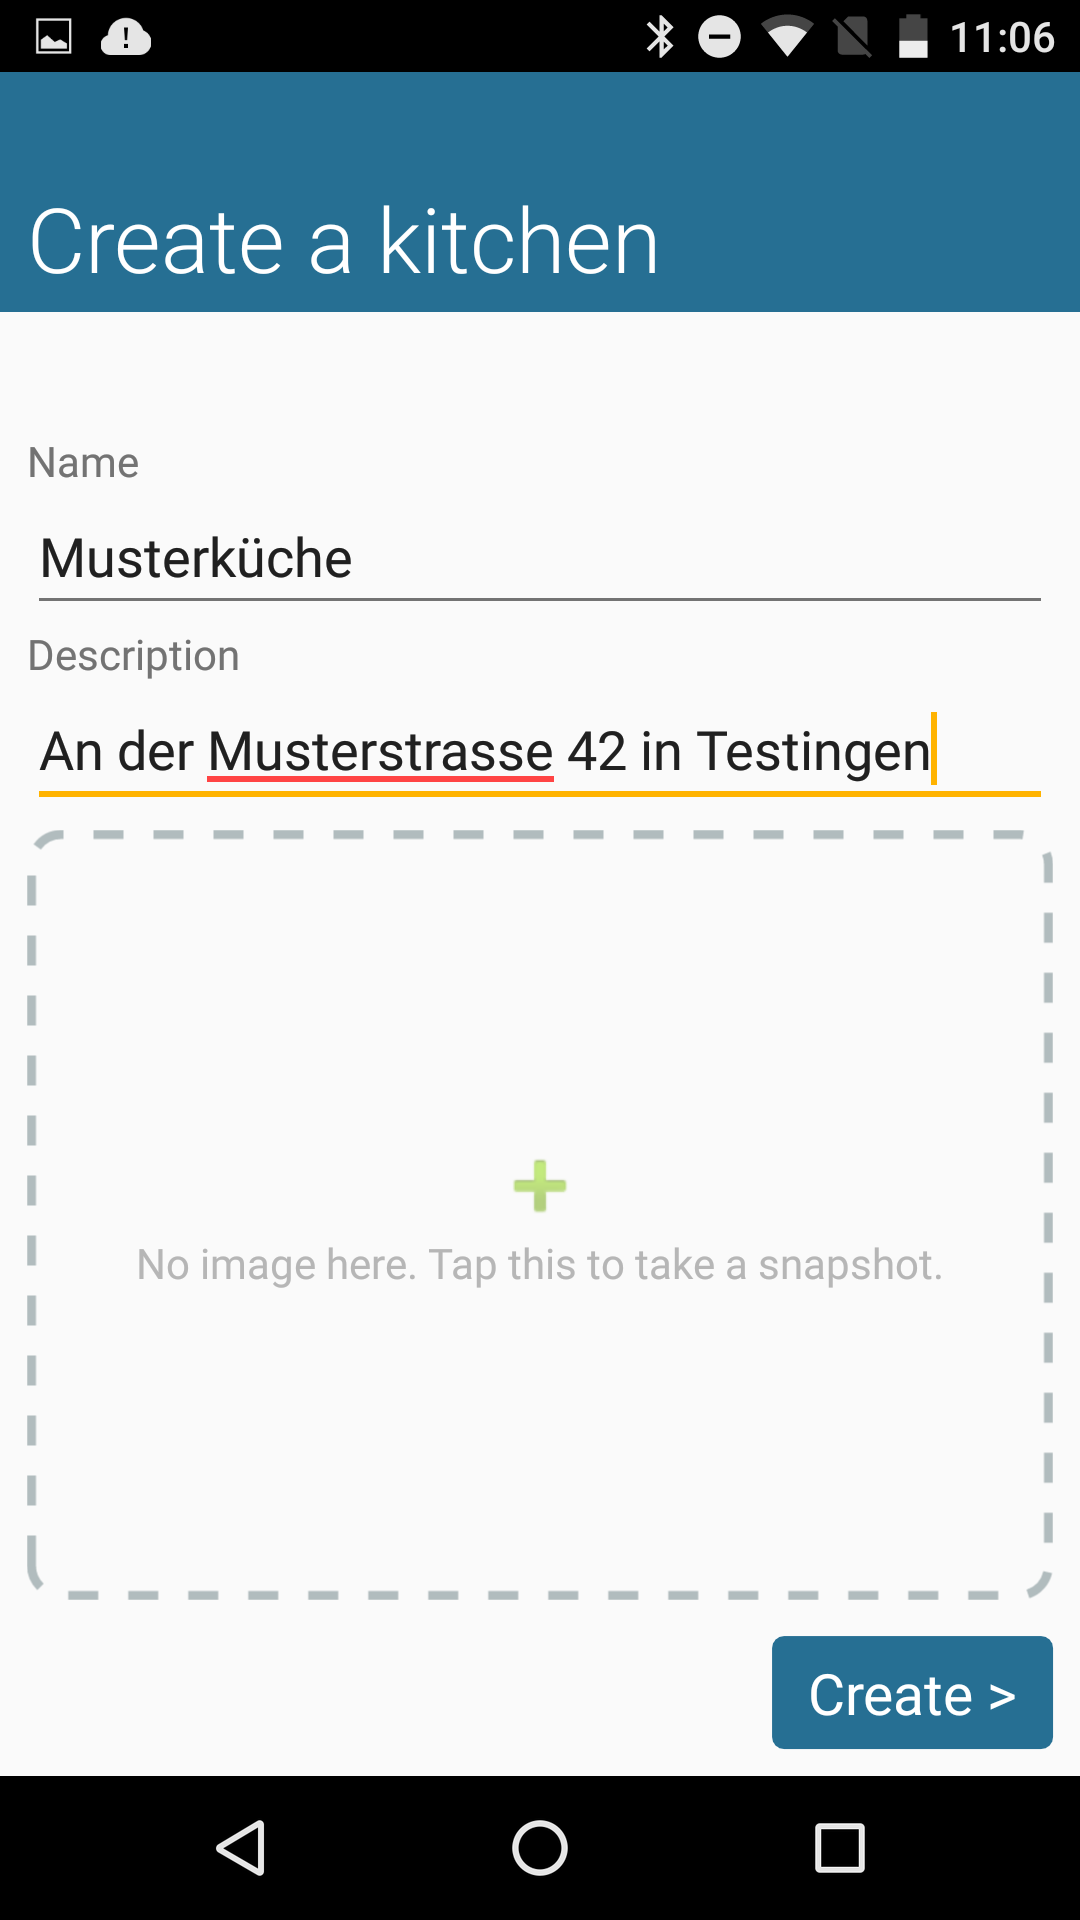
\includegraphics[scale=0.13]{results/res/create_kitchen}
	\caption{Küche erstellen}
\end{wrapfigure}
Dies öffnet die Applikationseinstellungen, wo Nutzername und das Passwort eingegeben werden können.\footnote{Zu Testzwecken kann der Benutzername: \enquote{user} und das Passwort: \enquote{1234} verwendet werden.}

\subsection{Küche erfassen}
Um eine Küche zu erfassen, berührt man den \acl{FAB} in der unteren rechten Ecke der Ansicht \enquote{Find a kitchen}. Danach wird der Name der Küche sowie eine optionale Beschreibung erfasst. Zum Schluss wird noch ein Foto der Küche erstellt, um eine schnelle Wiedererkennung zu ermöglichen.

Nun können für die neu erstellte Küche verschiedene Küchenbereiche erfasst werden. Dazu wird in der aktuellen Ansicht der \acl{FAB}

\WFclear
in der unteren rechten Ecke berührt. Dies kann so lange wiederholt werden, bis alle Bereiche der Küche erfasst wurden. 

\subsection{Suchlauf durchführen}

Nachdem eine Küche mit mindestens einem Küchenbereich erfasst wurde, können Geräte auf dem Bereich platziert werden. Dazu berührt man zuerst das Bild eines Küchenbereichs. Um in diesem Bereich nun einen Suchlauf durchzuführen, muss das Bluetooth Symbol in der oberen rechten Ecke berührt werden. Dieses öffnet eine Liste, welche nun laufend mit den gefunden Geräte befüllt wird. 

\begin{wrapfigure}{l}{5.5cm}
	\vspace{-0.44cm}
	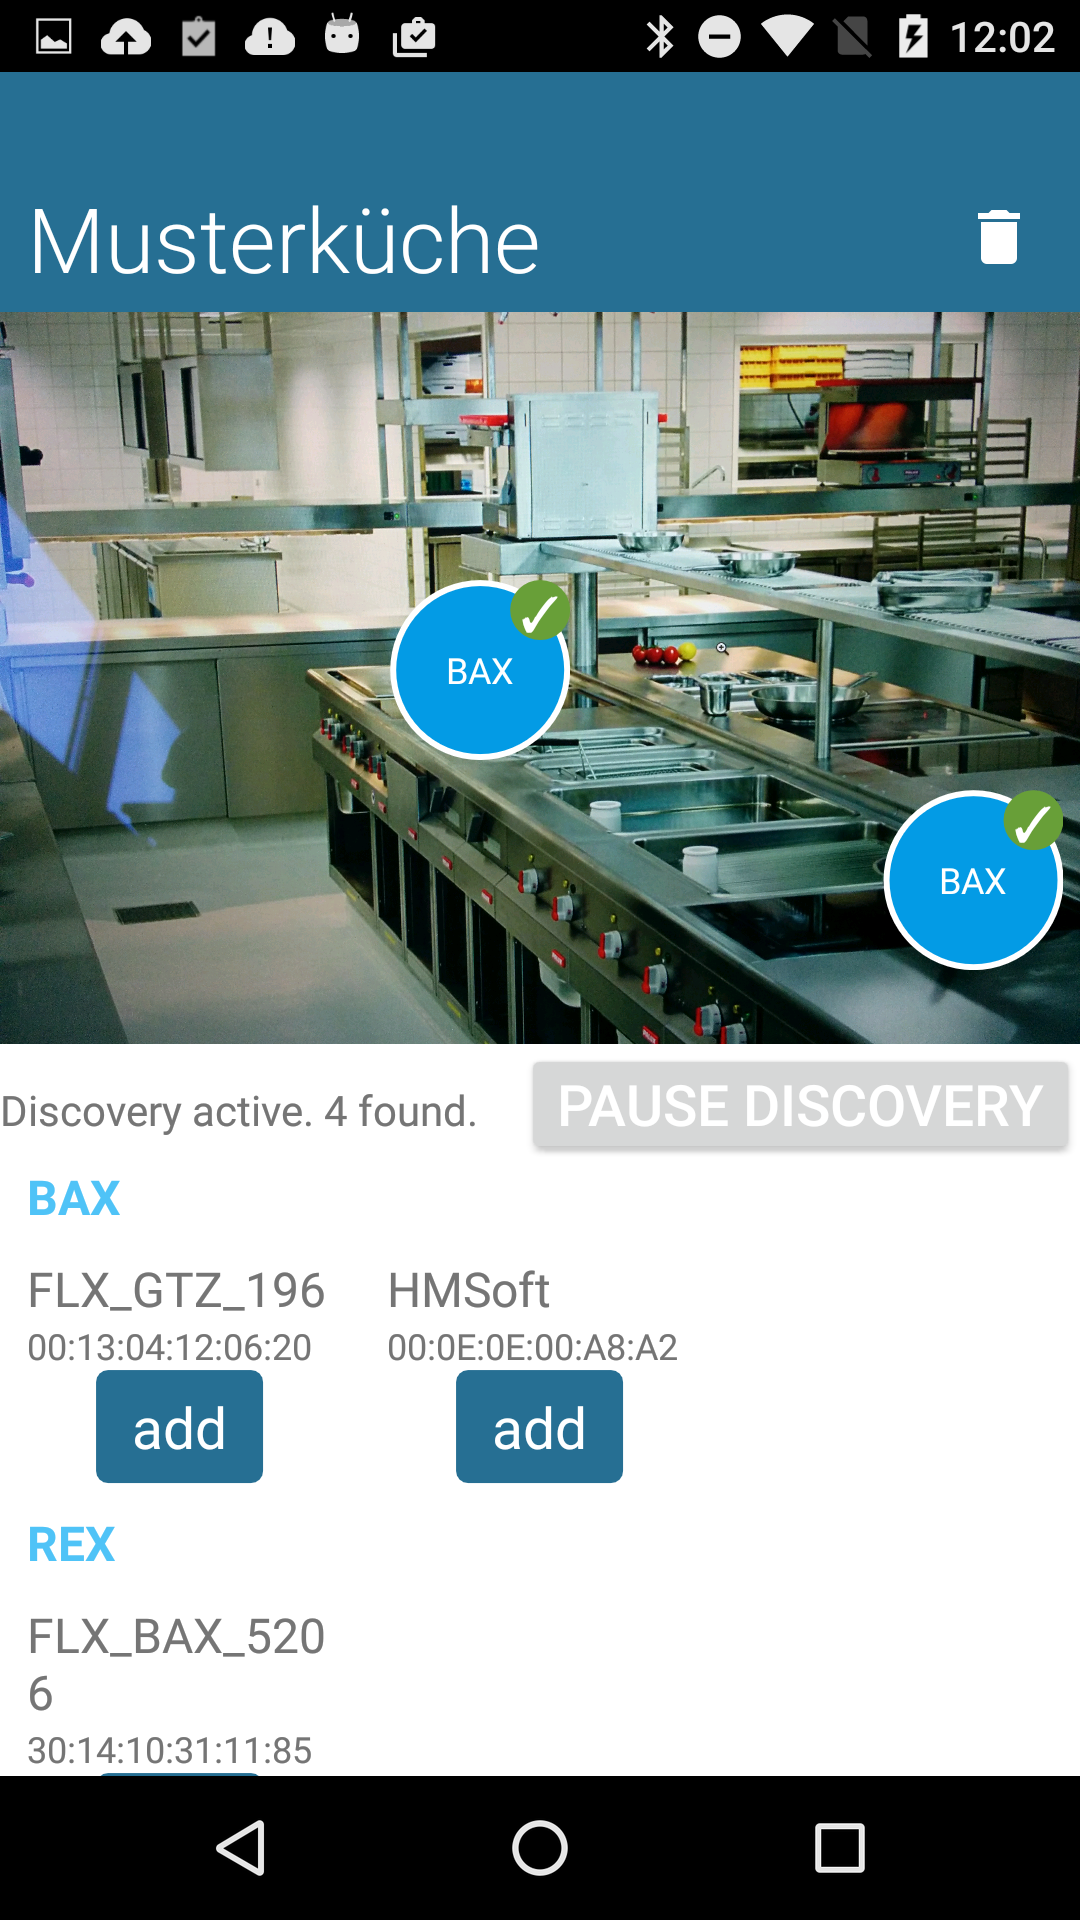
\includegraphics[scale=0.13]{results/res/device_discovery}
	\caption{Geräteerkennung}
\end{wrapfigure}

Geräte, mit denen noch keine Verbindung bestand, zeigen den Button \enquote{Pair} an. Damit wird der Bonding-Vorgang gestartet, welcher kurzzeitig ein Pop-Up für eine Passworteingabe anzeigt. Bei Geräten, die mit dem Default Passwort \enquote{1234} konfiguriert sind, muss nichts weiter gemacht werden, das Pop-Up verschwindet nach einigen Sekunden automatisch und der Button zeigt daraufhin \enquote{Add} an.

Nach dem Bonding-Vorgang können Geräte auf dem Küchenbereich platziert werden. Dazu berührt man den \enquote{Add} Button, worauf das Gerät in der Mitte der Ansicht erscheint. Das Gerät kann auf der Ansicht frei verschoben werden, so dass es mit der Einrichtung der Küche übereinstimmt. 

Sobald alle Geräte erfolgreich platziert wurden, kann der \enquote{Discovery Modus} mit dem Backbutton des Smartphones verlassen werden.

\WFclear
\subsection{Gerätestatus abrufen}
Um den Status eines Geräts abzurufen, muss man sich in der Küchenbereichsansicht befinden. Danach öffnet eine Berührung des gewünschten Geräts die Geräteansicht. Hier hat man die Wahl zwischen vier Tabs: Status, Usage, Errors und Config.

\begin{figure}[h!]
\centering
    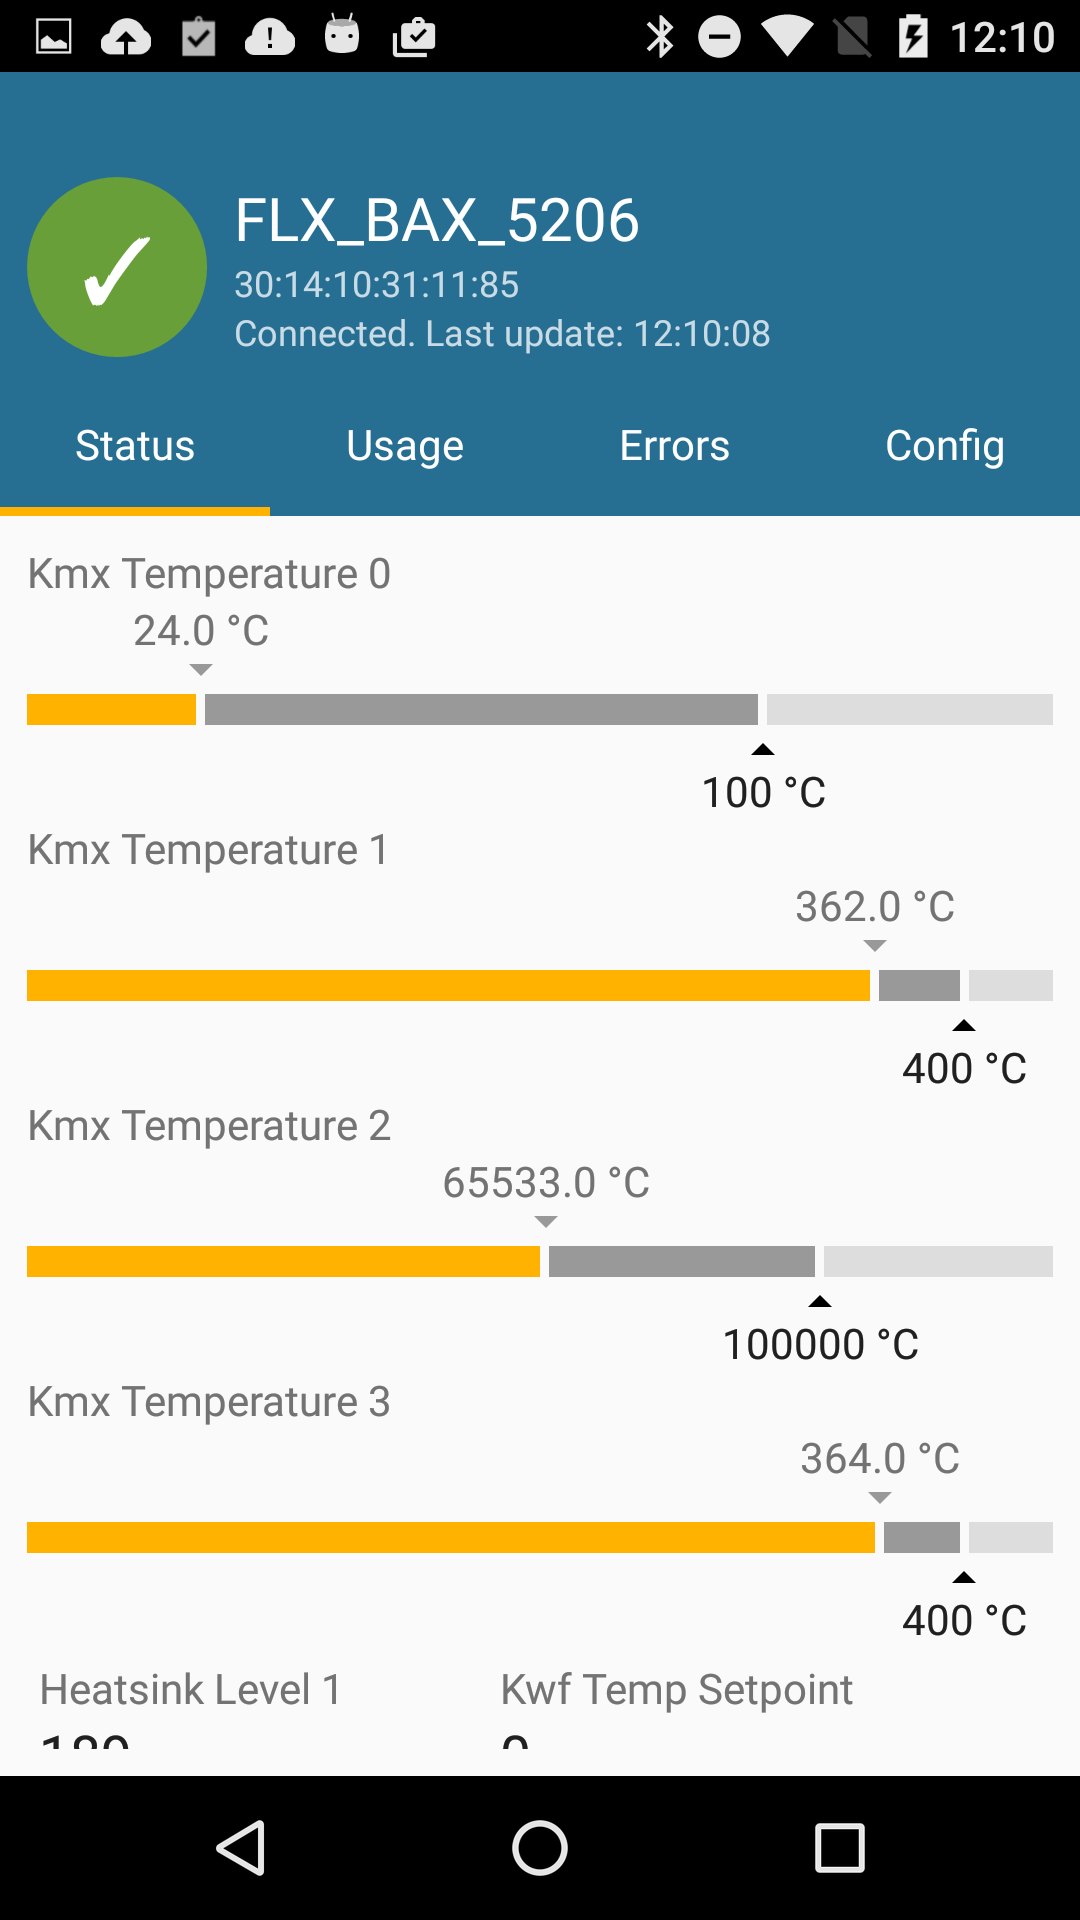
\includegraphics[scale=0.09]{results/res/device_status}
    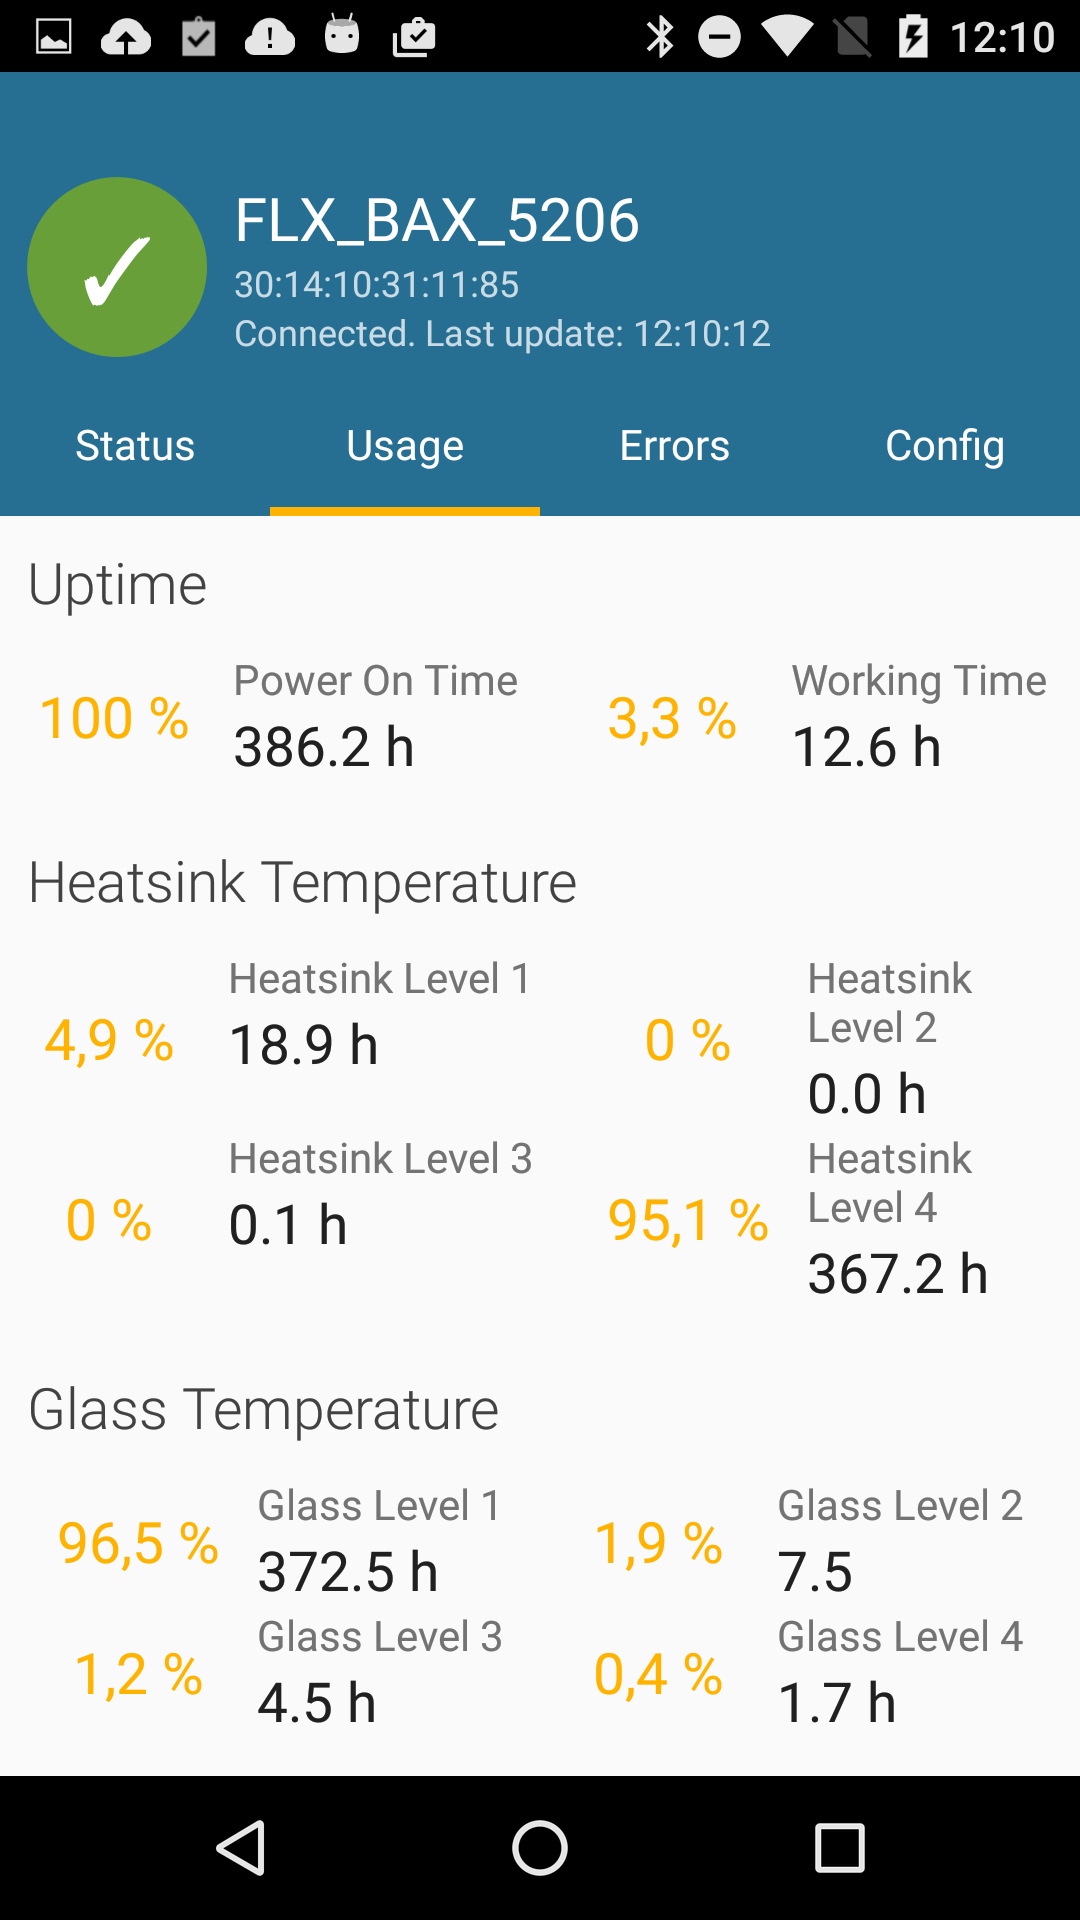
\includegraphics[scale=0.09]{results/res/device_usage}
    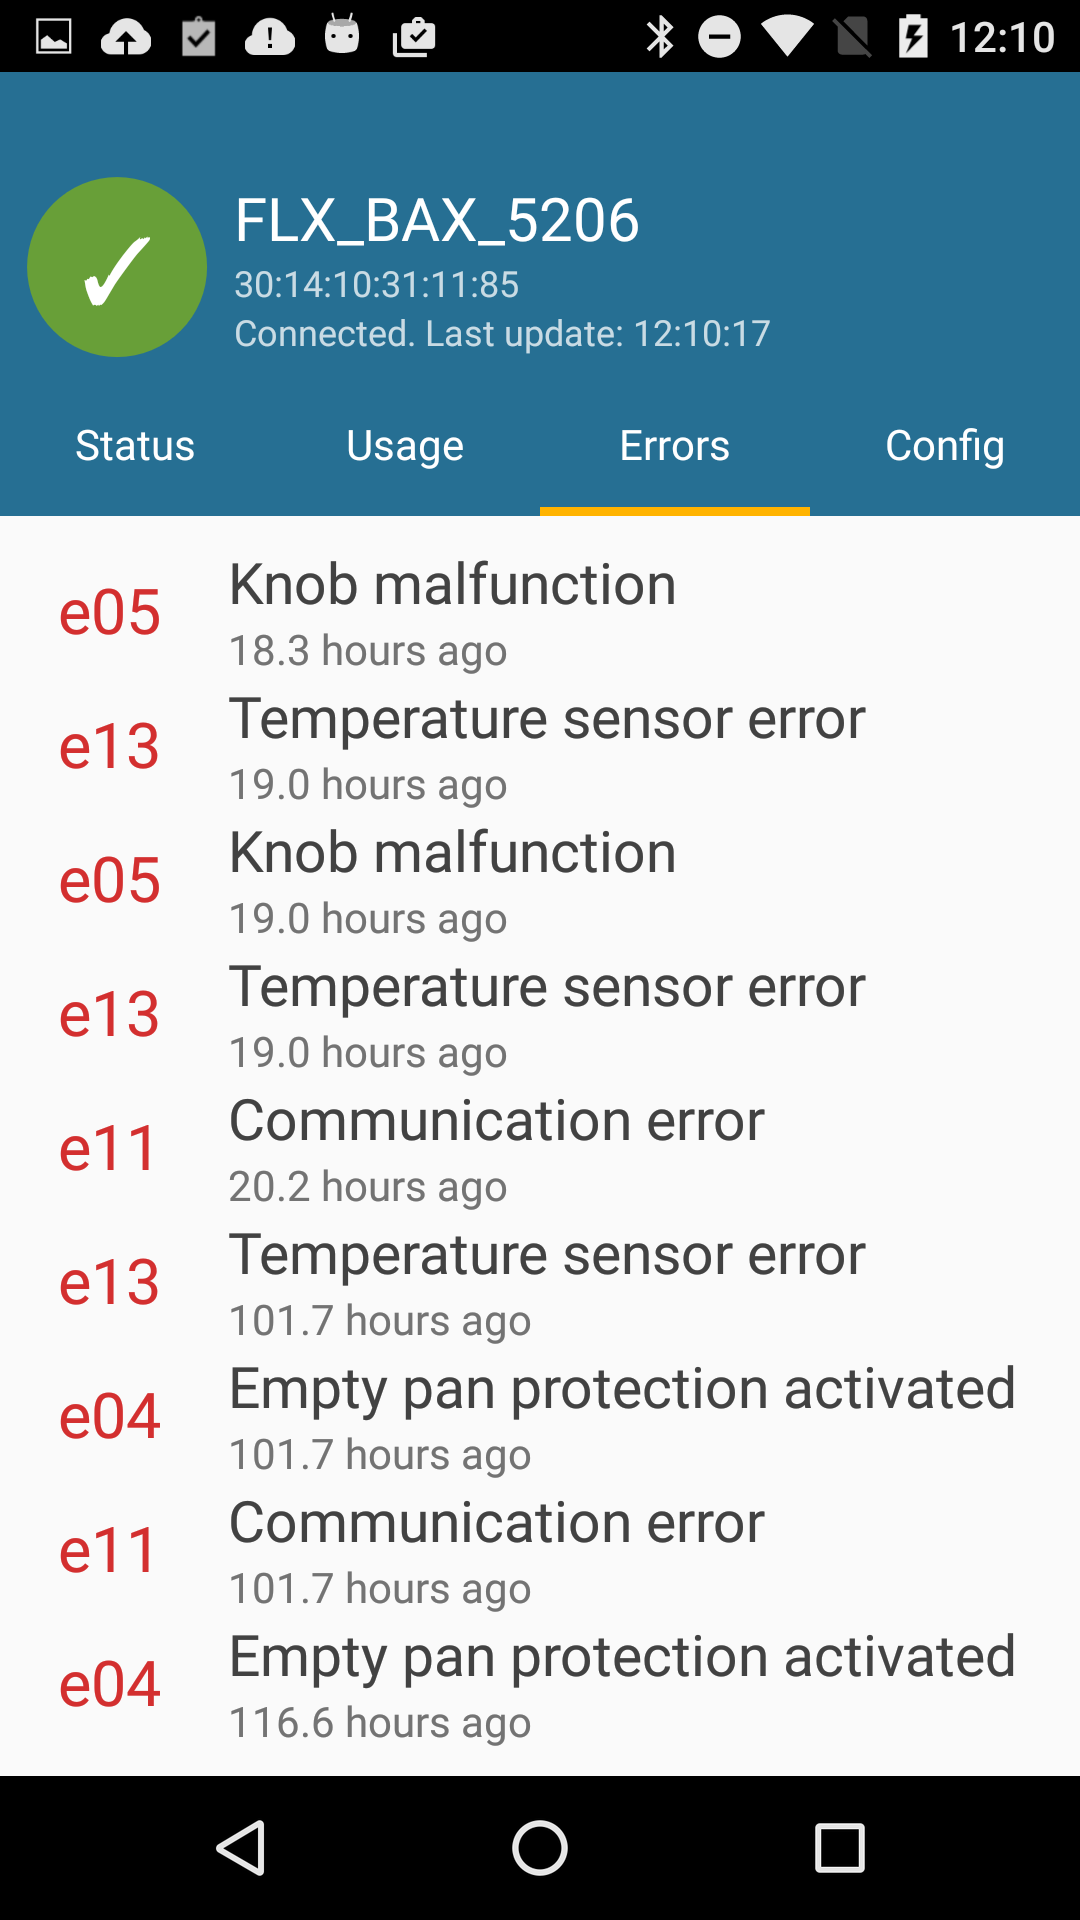
\includegraphics[scale=0.09]{results/res/device_errors}
    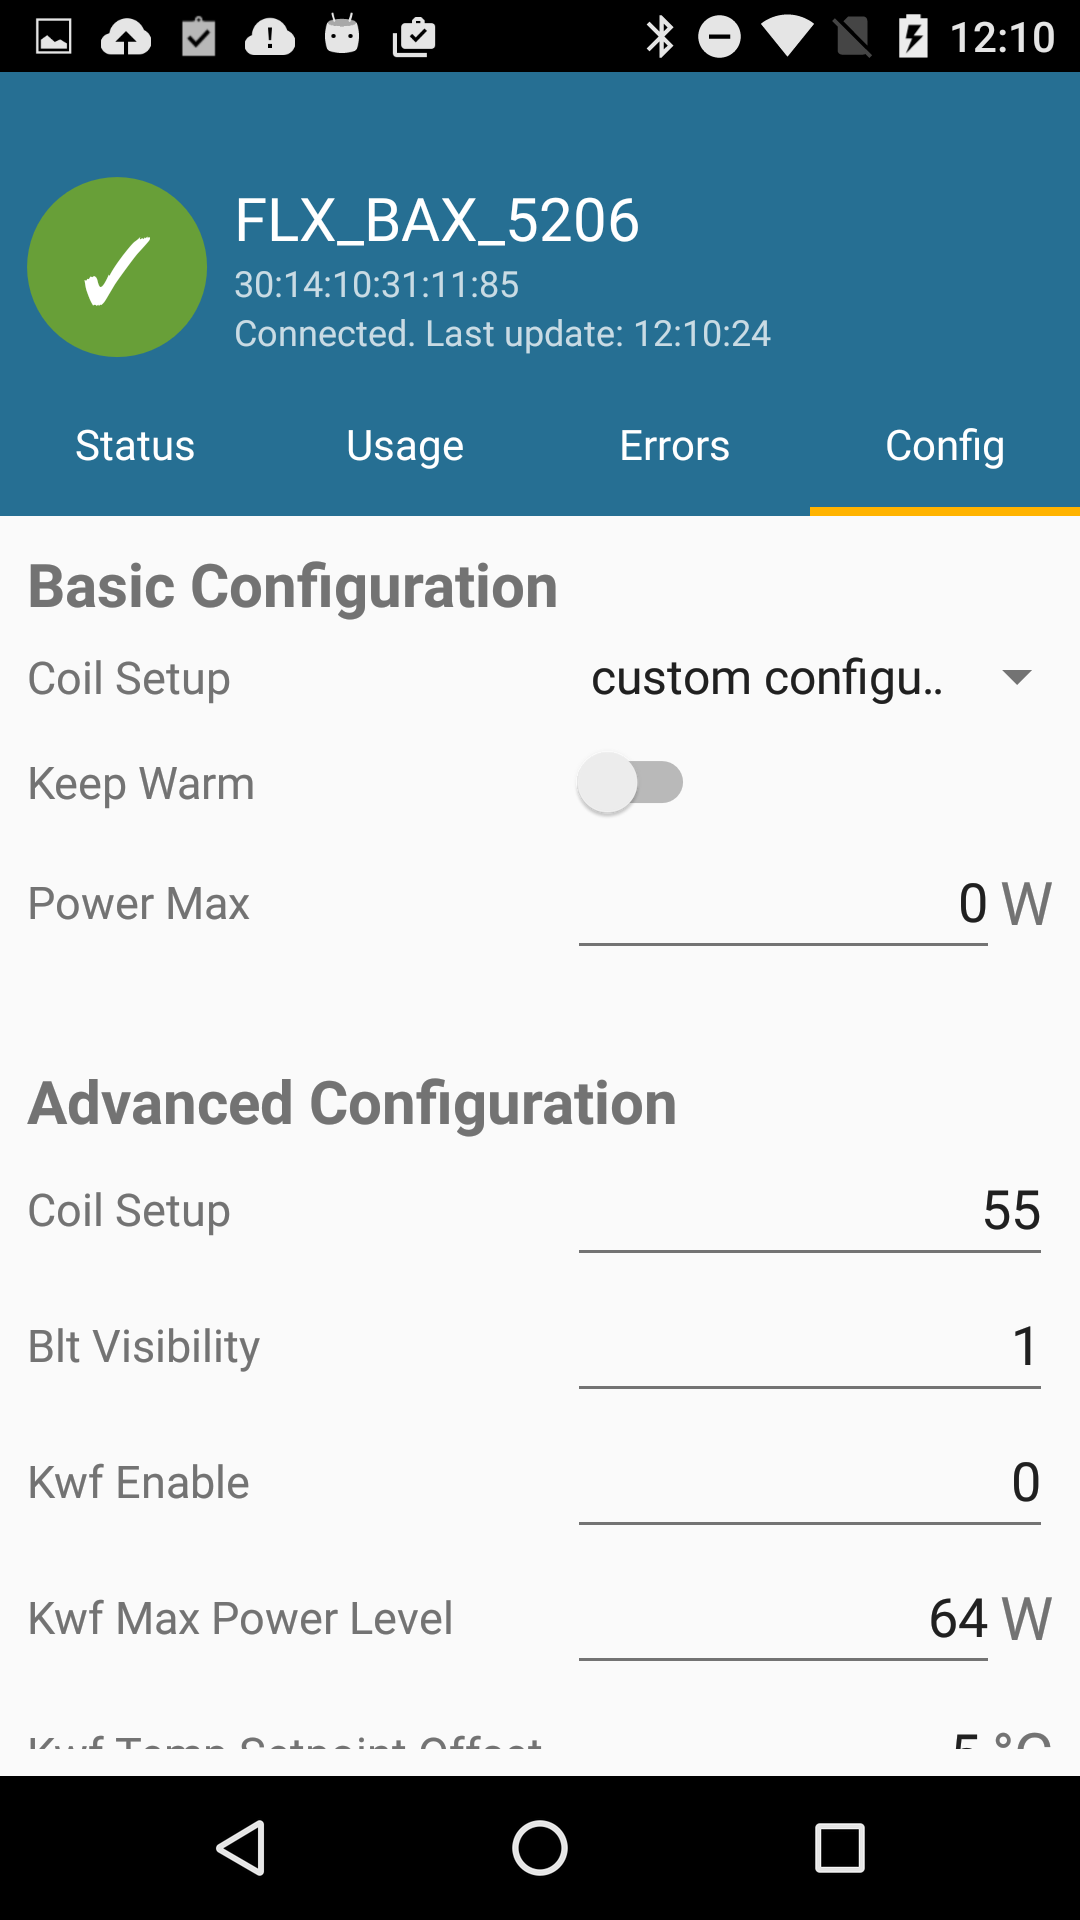
\includegraphics[scale=0.09]{results/res/device_config}
    \caption{Geräte-Detailansicht}
\end{figure}

\begin{itemize}
\item \textbf{Status:}
In der Statusansicht wird die aktuelle Temperatur aller angeschlossenen Sensoren angezeigt. \\
\item \textbf{Usage:}
Unter Usage findet man die Uptime des Geräts sowie die Benutzungsdauer einiger der wichtigsten Komponenten. \\

\item \textbf{Errors:}
Der Tab Errors zeigt eine Liste der Fehler die auf dem Gerät aufgetreten sind. \\

\item \textbf{Config:}
Unter Config können Geräteinstellungen eingesehen und verändert werden. Config ist in eine Überschrift \enquote{Basic Configuration} mit nur den nötigsten Einstellungen sowie \enquote{Advanced Config} mit allen Einstellungen gegliedert.
\end{itemize}

\WFclear
\subsection{Küche editieren}
\label{subsec:kuecheEditieren}
Ausgehend vom Screen \enquote{Find a kitchen} wird eine Küche gewählt und auf das Zahnrad in der oberen rechten Ecke gedrückt. Dies öffnet die Kücheneinstellung, in welcher der Name und die Beschreibung der Küche geändert werden können. Änderungen werden automatisch gespeichert.

\subsection{Küche exportieren}
\label{subsec:kuecheExportieren}
Um eine Küche zu exportieren muss zuerst zu den Kücheneinstellungen navigiert werden (siehe \ref{subsec:kuecheEditieren}). Dort kann via dem Button \enquote{Share via EMail} der Export-Vorgang gestartet werden. Nachdem die Applikation den Export zusammengestellt hat, erscheint eine Auswahl von Applikationen mit denen die exportierte Küche versendet oder gespeichert werden kann. Wenn zum Beispiel Gmail gewählt wird, wird die exportierte Küche als .fluxron Datei angehängt. 

\subsection{Küche importieren}
Um eine Küche zu importierten, benötigt man eine .fluxron Datei (siehe \ref{subsec:kuecheExportieren}). Diese Datei kann auf ein Smartphone via File Transfer übertragen und dann mit einem herkömmlichen Datei Explorer geöffnet werden. Alternativ kann man sich Datei auch als EMail Anhang zusenden und direkt aus der Mail Applikation heraus öffnen.

\subsection{Deinstallation}
Die Deinstallation erfolgt durch ein langes Drücken des Applikationsicons. Das Icon kann dann auf den Mülleimer gezogen werden, der am oberen Bildschirmrand erscheint. Alternativ kann die Applikation auch in den Android-Einstellungen unter \enquote{Apps} deinstalliert werden.
\chapter{Ausblick}
\label{chap:Ausblick}

\section{Weiterentwicklungsmöglichkeiten}
\label{sec:Weiterentwicklungsmöglichkeiten}

\subsection{Kommunikation mit weiteren Gerätetypen}
\label{subsec:KommTypen}

In der aktuellen Version der App wurden nur die Gerätetypen C- und S-Class vollständig angebunden. Zukünftig sollten aber auch weitere Fluxron-Geräte angesprochen werden können.

Dies wird von unserer App bereits konzeptionell unterstützt, d.h. es müssen lediglich die Benutzeroberflächen für die entsprechenden Gerätetypen gezeichnet werden. Je nach Gerätetyp muss auch noch die Code-Generierung um die entsprechenden Parameterdateien erweitert werden. Die App unterscheidet die Geräte bereits an ihrem Herstellercode und kann daher um beliebige Gerätetypen erweitert werden.

\subsection{Internet- / Cloudanbindung}
\label{subsec:Internetanbindung}

Da die Anwendung typischerweise von Angestellten einer Servicefirma genutzt wird, ist die aktuelle Möglichkeit, Küchen via E-Mail auszutauschen nicht langfristig praktikabel. Daher wird eine Internetanbindung der App zusätzlichen Nutzen verleihen. Die Firmen könnten damit die erfassten Küchen an alle Mitarbeiter verteilen und müssten sich nicht mehr um eine Datensicherung der einzelnen Geräte kümmern. Zudem wäre die Verwaltung aller Küchen einer Servicefirma über ein Webportal denkbar.

Aber nicht nur für die Servicefirmen hätte eine solche internet- bzw. cloubasierte Lösung Vorteile. Auch die Firma Fluxron könnte von dieser profitieren. Es könnten zusätzliche Einnahmen mit dem Vermieten des Cloudservers an die Servicefirmen erzielt werden.

Eine solche Anbindung ist mit der von uns gewählten Applikationsarchitektur problemlos möglich. Dabei kann einerseits die Datenbank (Couchbase Lite) mit einem Cloud-Backend verbunden werden. Dies ist von Couchbase bereits im Rahmen von Merge-Replikation unterstützt und ist damit mit geringem Aufwand möglich.

Mit etwas mehr Entwicklungsaufwand könnte aber auch eine komplett neue Komponente zur Internetanbindung and den Daten-EventBus angehängt werden. Diese würde dann die empfangenen Meldungen an ein Cloud-Backend weiterleiten und damit theoretisch sogar eine Echtzeitanbindung ermöglichen.

\subsection{Erstellen eines Geräteabbilds}
\label{subsec:WeiterleitenVonFehlern}

Ähnlich der momentanen Exportmöglichkeit für Küchen, wäre eine Erweiterung der App denkbar, welche es erlaubt, ein Abbild eines Gerätes zu erstellen. Dieses Geräteabbild könnte die Fehlerhistorie, Nutzungsstatistiken und alle Parameter (mit Werten) des Gerätes enthalten. Danach könnte das exportierte Abbild an die Herstellerfirma gesendet werden, um eine Fehlerdiagnose zu machen.

Neben dem Export eines Geräteabbildes wäre natürlich auch der Import eines Geräteabbildes von Nutzen. So könnten Mitarbeiter der Firma Fluxron Konfigurationen vor Ort vom Handy auf mehrere Geräte überspielen oder die Konfiguration an eine Servicefirma weiterleiten, welche dann die Einstellungen auf die beim Kunden installierten Geräte übertragen kann.

\subsection{Erhebung von Nutzungsprotokollen}
\label{subsec:Nutzungsprotokolle}

Verbindet man die Cloudanbindung (\ref{subsec:Internetanbindung}) und die Erstellung von Geräteabbildern (\ref{subsec:WeiterleitenVonFehlern}) wäre auch eine Erhebung von Nutzungsprotokollen der Geräte möglich. Damit kann die Firma die Leistung der Geräte dem Kundenbedarf anpassen und optimieren.

Ausserdem könnten auch die Servicefirmen von einer solchen Erhebung profitieren. Sie können so einfacher Probleme diagnostizieren und Support für ihre Kunden anbieten. Häufig bauen die Servicefirmen die Fluxron-Geräte in eigene Küchenkombinationen ein, welche dann weiterverkauft werden. Mittels der Nutzungsstatistik kann so der Marktbedarf besser eingeschätzt werden.

Ein weiterer Nutzen der Statistiken wäre es, Vorhersagen über mögliche nahende Probleme eines Gerätes machen zu können. So könnten die Geräte ausgetauscht oder repariert werden, bevor die Probleme im laufenden Betrieb auftreten.

\nocite{*}
\bibliographystyle{IEEEtran}
\bibliography{Fluxron}


% \acs prints the longform the first time, after that the short
% using \ac always prints the shortform
   
\chapter*{List der Abkürzungen}\addcontentsline{toc}{chapter}{List of
Abbreviations}
\begin{acronym}[SPARC] % [] should contain the longest acronym
    \acro{API}{Application Programming Interface}
    \acro{CI}{Continuous Integration} 
	\acro{ECTS}{European Credit Transfer and Accumulation System}
	\acro{IDE}{Integrated Development Environment}
	\acro{JAR}{Java ARchive file}
	\acro{JVM}{Java Virtual Machine}
	\acro{HSR}{Hochschule für Technik Rapperswil}
	\acro{PDF}{Portable Document Format}
	\acro{TDD}{Test Driven Delevopment}
	\acro{UI}{User Interface}
	\acro{URL}{Uniform Resource Locator}
	\acro{VM}{Virtual Machine}
	\acro{XML}{Extensible Markup Language}
	\acro{LE}{Low Energy}
	\acro{FR}{Functional Requirement}
	\acro{NFR}{Non Functional Requirement}
\end{acronym}


\cleardoublepage
\phantomsection
\addcontentsline{toc}{chapter}{\listfigurename}
\listoffigures

\cleardoublepage
\phantomsection
\addcontentsline{toc}{chapter}{\listtablename}
\listoftables

% Summary index document for the appendix
\appendix
\pagenumbering{Roman}
\renewcommand{\thesection}{\Alph{section}}

%\setcounter{table}{0}
\renewcommand{\thetable}{\Alph{section}.\arabic{table}}
\renewcommand\thefigure{\Alph{section}.\arabic{figure}}

\
\addcontentsline{toc}{chapter}{Anhang}
\chapter*{Anhang}

%Anhänge hier
\section{Infrastruktur}
\label{Infrastruktur}

\subsection{Entwicklungsumgebung}
Als \ac{IDE} wurde für dieses Projekt Android Studio 1.4 eingesetzt. Android Studio basiert auf IntelliJ und hat Ende 2014 die \enquote{Eclipse Android Development Tools} als Standard \ac{IDE} für Android Projekte abgelöst.\cite{android_studio_stable}

Für die Versionsverwaltung wurde Git mit einem Projekt Repository der \ac{HSR} (\url{git.hsr.ch}) verwendet. Lokal wurde der grafische Git-Client SourceTree benutzt.

Um Continuous Integration zu ermöglichen haben wir zusätzlich auf einem \ac{VPS} der \ac{HSR} einen Jenkins Build-Server eingerichtet. Der Build-Server prüft mittels Polling ob neue Commits vorhanden sind und kompiliert gegebenenfalls jeweils eine neue Version der Applikation. So wird sichergestellt, dass eine Änderung nicht nur lokal kompiliert, sondern überall. Zudem bietet der Build-Server die Möglichkeit, die jeweils aktuellste Version der Applikation an Tester zu verteilen.

\subsection{Projektmanagement}

Zur Unterstützung des Projektmanagements wurde Redmine auf dem \ac{VPS} der \ac{HSR} eingerichtet. Vor allem die von Redmine gebotenen Funktionen Issue Verwaltung, Gantt Diagramm, Wiki und File-Repository wurden intensiv eingesetzt.

\subsection{Testgeräte}

Von der \ac{HSR} wurden uns zwei Android Smartphones zur Verfügung gestellt. Ein \enquote{LG Nexus 5} mit Android 6.0 sowie ein \enquote{Samsung Galaxy Nexus} mit Android 4.3. Mit dem \enquote{Samsung Galaxy Nexus} decken wir die Mindestanforderungen der Applikation (API Level 18 - Android 4.3) ab und mit dem \enquote{LG Nexus 5} wird sichergestellt dass die Applikation auch auf Geräten mit der neusten Android Version (Stand Dezember 2015) läuft.

Zum simulieren der Küchengeräte erhielten wir von Fluxron einen Testaufbau. Dieser besteht aus drei Bluetooth Controllern wie sie bei Induktionsheizgeräten eingesetzt werden.

\begin{wrapfigure}[15]{l}{9cm}
	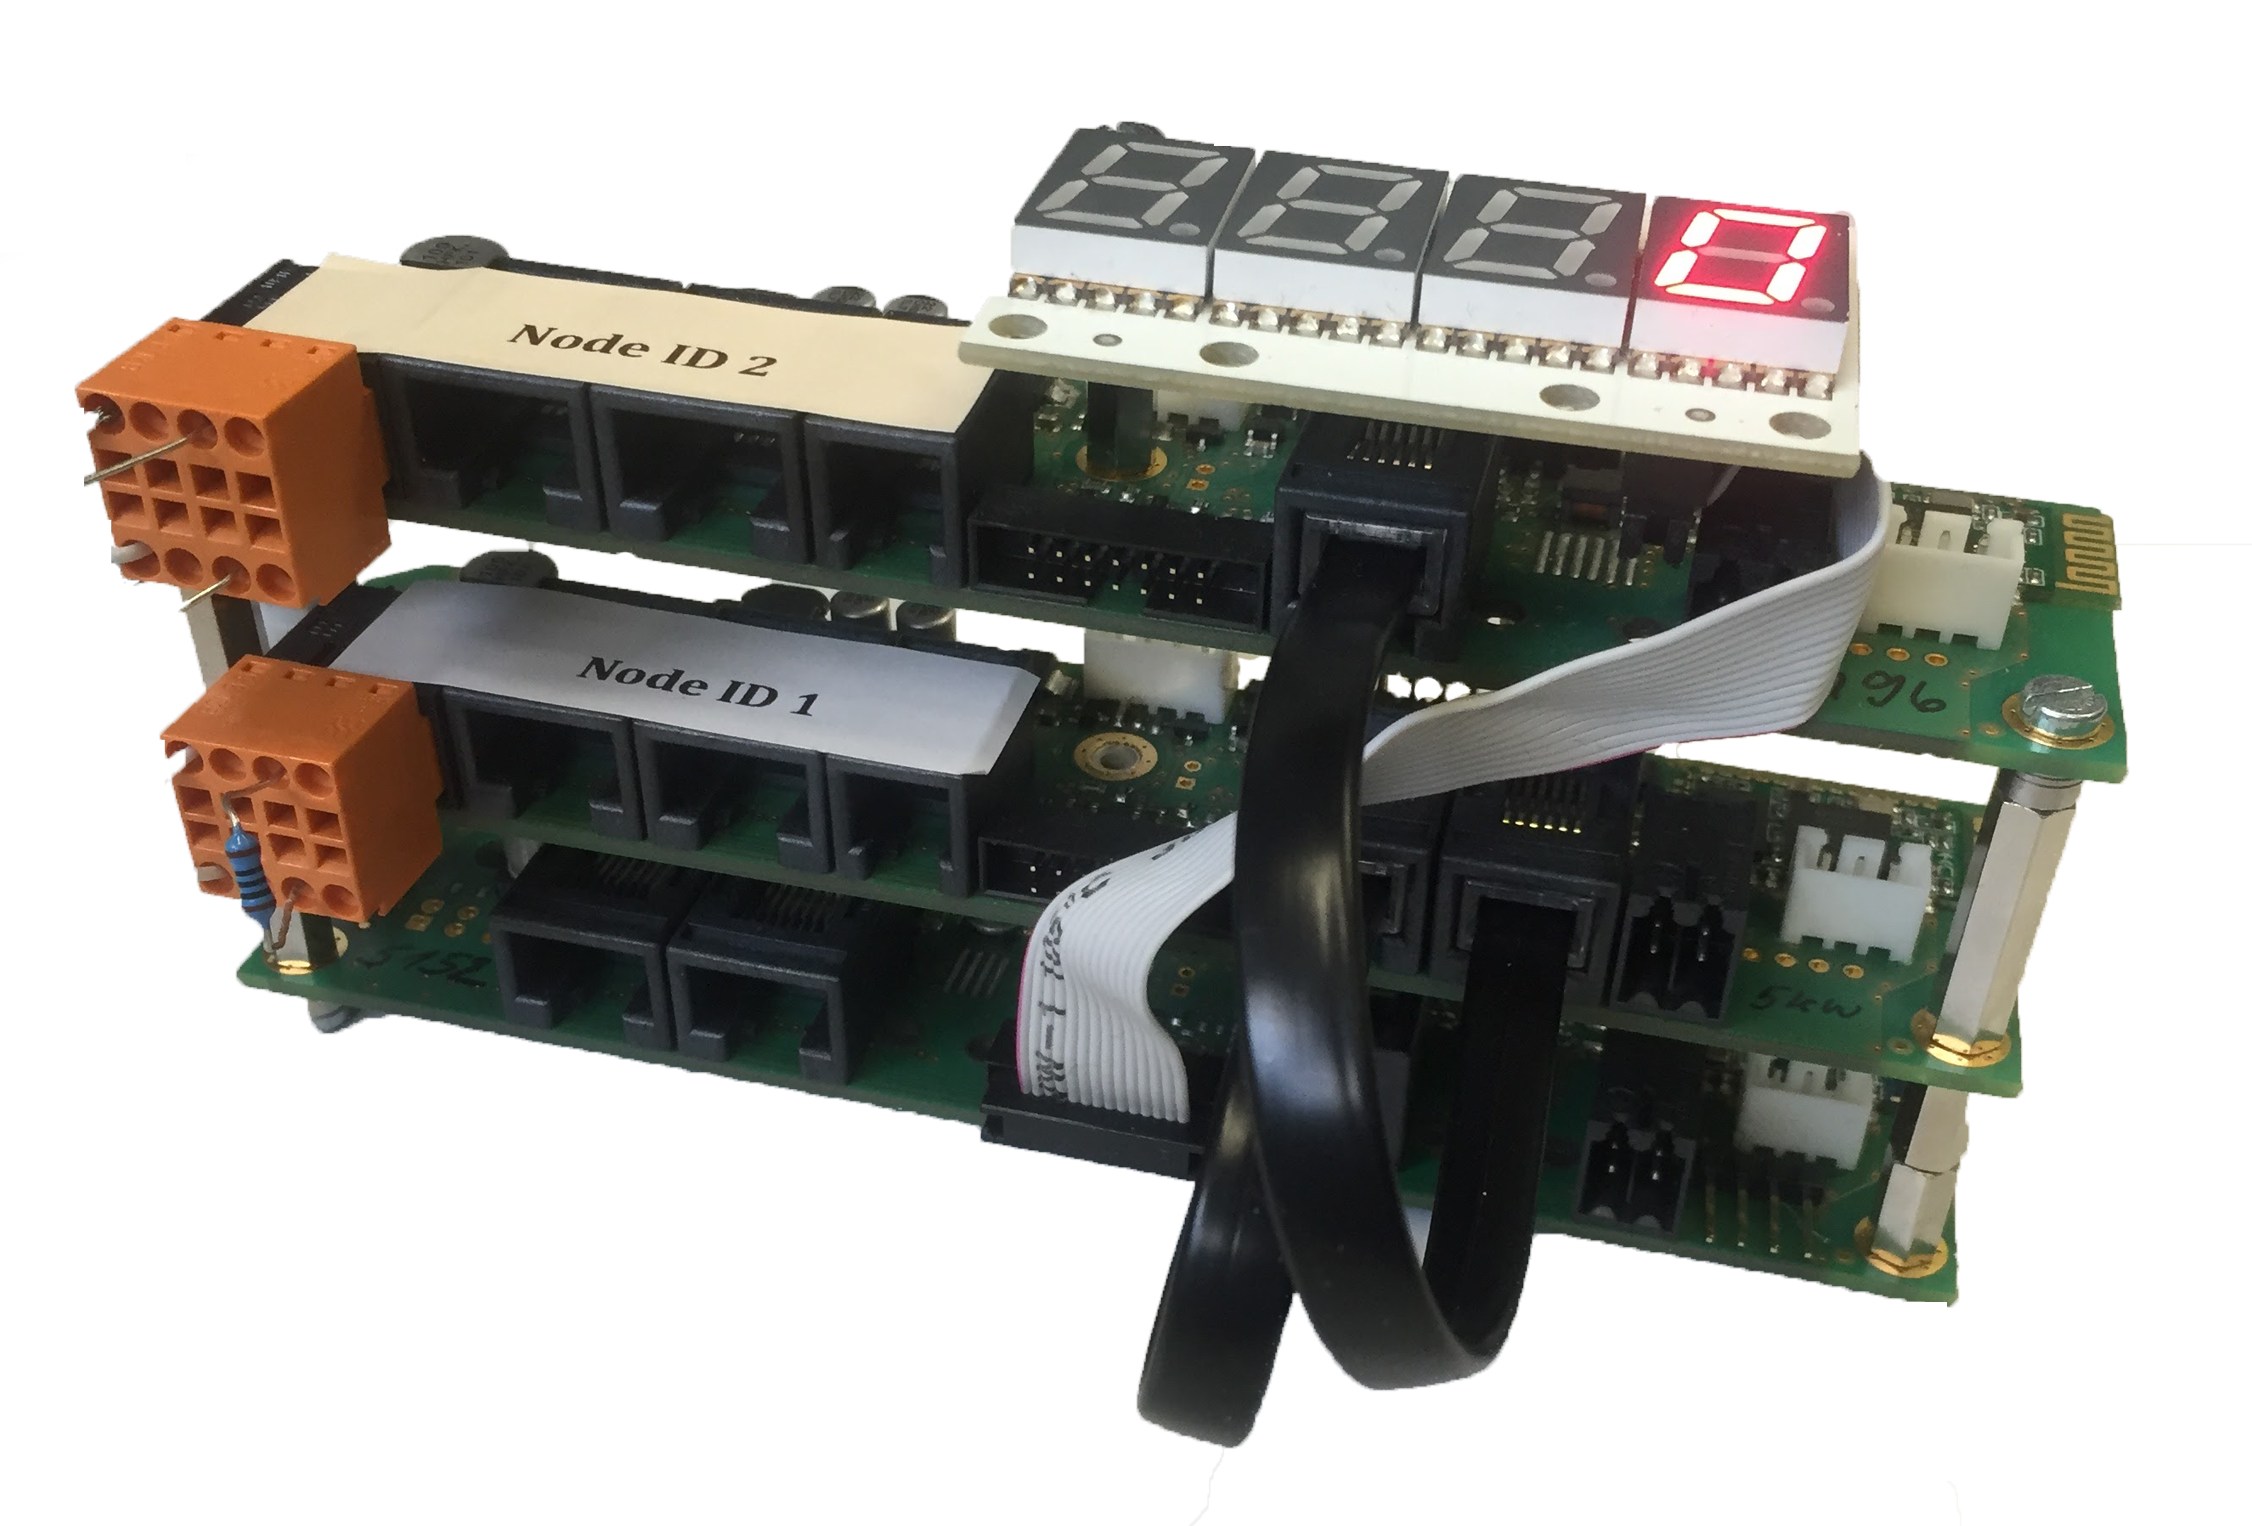
\includegraphics[scale=0.1025]{appendix/res/fluxron_device_transparent}
	\caption{Fluxron Testaufbau}
\end{wrapfigure}

\ 

\begin{enumerate}
\item \textbf{Revision:} C-Class\\ \textbf{Typ:} BAX\\ \textbf{Bluetooth:} Classic\\
\item \textbf{Revision:} C-Class\\ \textbf{Typ:} REX\\ \textbf{Bluetooth:} Classic\\
\item \textbf{Revision:} C-Class\\ \textbf{Typ:} BAX\\ \textbf{Bluetooth:} Classic \& 4.0
\end{enumerate}
